\documentclass[12pt]{article}

%\renewcommand{\baselinestretch}{1.65}
\usepackage{amsmath,graphicx,bbm,amssymb}
\usepackage{txfonts}
\usepackage{array}
\usepackage{subfigure}
\usepackage{ccaption}
\usepackage{xcolor}
\usepackage{tikz}
\usetikzlibrary{arrows} 
\usetikzlibrary{shapes.multipart}
\usetikzlibrary{shapes.misc, positioning}
\usepackage{float}
\usepackage{calc}
\usepackage{multirow}
\usepackage{fancyhdr}
\usepackage{fancyvrb}
\usepackage{colortbl}
\usepackage[hmargin=1.5cm, top=2cm, bottom=2cm]{geometry}

\newcommand{\procspie}{Proc. SPIE } 
\newcommand{\pasp}{Publications of the Astronomical Society of the Pacific } 
\newcommand{\aap}{Astron. \& Astrophys. } 
\newcommand{\mnras}{M.N.R.A.S } 

\newcommand{\module}[1]{\left\vert #1 \right\vert}
\newcommand{\norme}[1]{\left\vert\left\vert #1 \right\vert\right\vert}
\newcommand{\para}[1]{\left(#1\right)}
\newcommand{\cro}[1]{\left[#1\right]}
\newcommand{\aver}[1]{\left\langle #1 \right\rangle}
\newcommand{\bra}[1]{\left\lbrace #1 \right\rbrace}
\newcommand{\xth}[1]{#1^{\text{th}}}
\newcommand{\otfdl}{\text{OTF}_\text{DL}}

\newcommand{\rz}{r_0}
\newcommand{\lz}{L_0}
\newcommand{\cnh}{C_n^2(h)}
\newcommand{\nwfs}{\text{n}_\text{wfs}}
\newcommand{\R}{\boldsymbol{\text{R}}}
\newcommand{\Mc}{\boldsymbol{\text{M}_c}}
\newcommand{\thSrc}{\boldsymbol{\theta}_\text{src}}
\newcommand{\thGs}{\boldsymbol{\theta}_\text{gs}}
\newcommand{\thNgs}{\boldsymbol{\theta}_\text{ngs}}
\newcommand{\thLgs}{\boldsymbol{\theta}_\text{lgs}}
\newcommand{\rbb}{\boldsymbol{r}}
\newcommand{\rbun}{\boldsymbol{r}_1}
\newcommand{\rbdeux}{\boldsymbol{r}_2}
\newcommand{\rhob}{\boldsymbol{\rho}}
\newcommand{\TTout}{\boldsymbol{\text{TT}}_\text{out}}
\newcommand{\TTonly}{\boldsymbol{\text{TT}}_\text{only}}
\newcommand{\codeline}[1]{\begin{Verbatim}[commandchars=\\\{\}]
		\textcolor{blue}{#1}
\end{Verbatim}}
\title{KASP Technical notes \#06:\\ Pupil model generator with KASP}
\author{G. Chataignier, O. Beltramo-Martin\footnote{olivier.martin@lam.fr}, C.~M. Correia}
\date{}


\setcounter{page}{1}
\fancyhead[LO,LE]{KASP Technical notes \#02}
\fancyhead[RE,RO]{O. Beltramo-Martin}
\pagestyle{fancy} 
\setlength{\parindent}{0cm}

\begin{document}
	
\maketitle	
\rule{\columnwidth}{0.1mm}
\tableofcontents
\rule{\columnwidth}{0.1mm}

\section{Purpose}
	
	
How to build a pupil using pupil and segment class


\section{Segment class definition}

\begin{par}
The segment class constructor has 3 required inputs :
\end{par} \vspace{1em}
\begin{itemize}
\setlength{\itemsep}{-1ex}
   \item Number of sides ( 3 : triangle, 6 : hexagon, inf : disk)
   \item External radius of a segment in meter (1.4/2 for eelt, 1.8/2 for Keck...)
   \item Definition in pixels for the matrix
\end{itemize}
\begin{par}
It also has optional inputs :
\end{par} \vspace{1em}
\begin{itemize}
\setlength{\itemsep}{-1ex}
   \item Angle in rad
   \item Coordinates in the pupil
   \item Reflexivity Error
   \item Coefficients for error phase modes
   \item Geometry errors : position, angle, size,
\end{itemize}
\begin{Verbatim}[commandchars=\\\{\}]
\textcolor{blue}{ S=segment(6,0.9,50); \% hexagon of 1.8 m, in a 50px matrix}
\end{Verbatim}
\begin{par}
Segment can be displayed via S.disp S.disp shows reflexivity and phase S.disp('r') shows reflexivity only S.disp('p') show phase only
\end{par} \vspace{1em}
\begin{Verbatim}[commandchars=\\\{\}]
\textcolor{blue}{S.disp;}
\end{Verbatim}

\begin{figure}
	\centering
	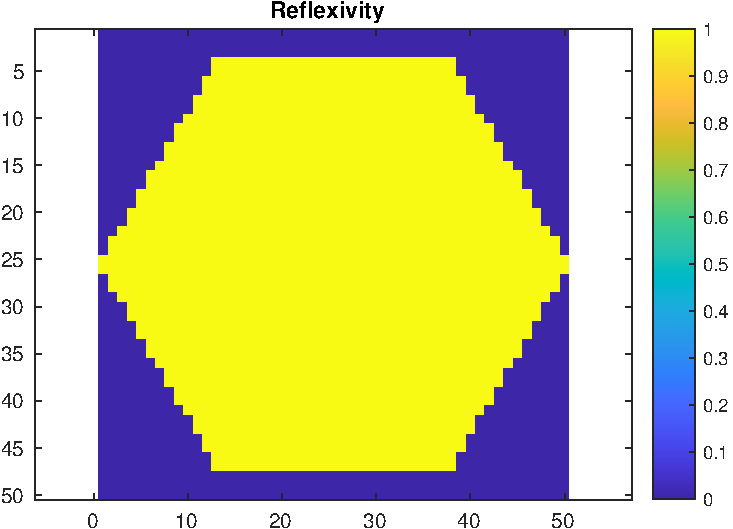
\includegraphics [width=3in]{docuPupilClass_01.pdf} \hspace{0.5cm}
	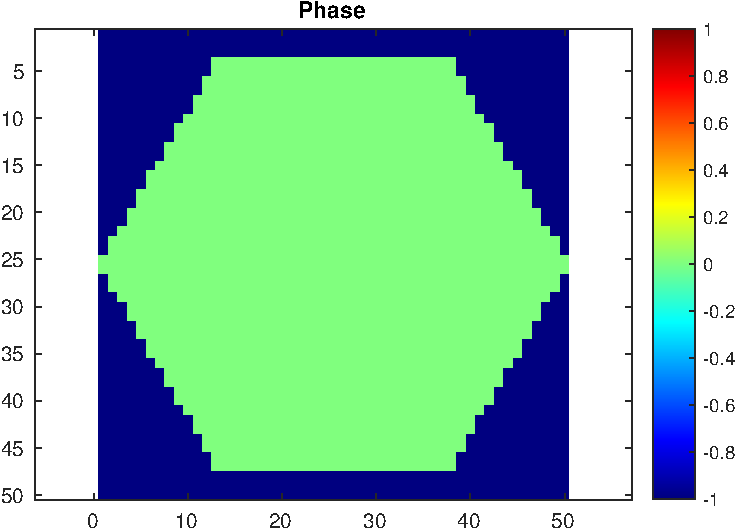
\includegraphics [width=3in]{docuPupilClass_02.pdf}
	\caption{Illustration of a segment}
\end{figure}



\subsection{Definition of a simple Pupil}

\begin{par}
The Pupil constructor has no Required input : It builds by default a circular telescope of 1 meter with no central obstruction represented in a matrix of 100 pixels.
\end{par} \vspace{1em}
\begin{verbatim}
P=pupil;
P.disp('r');
\end{verbatim}

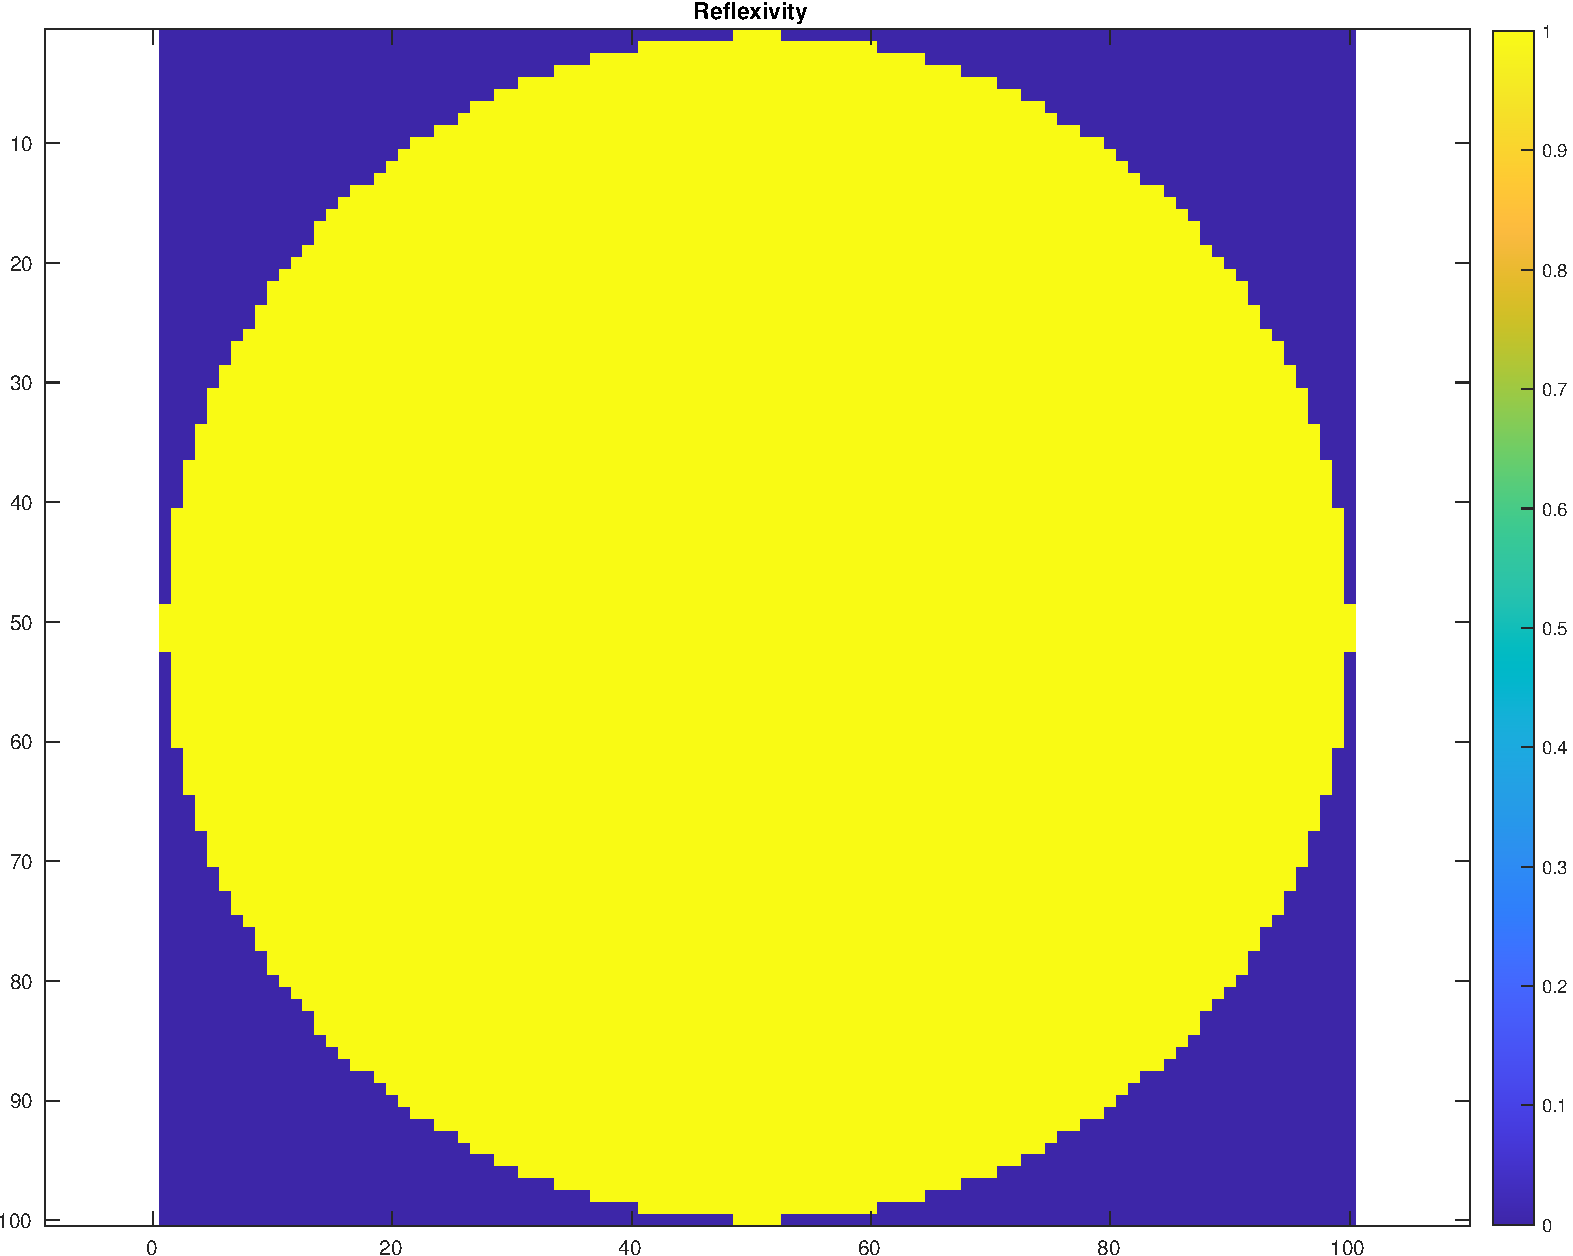
\includegraphics [width=4in]{docuPupilClass_03.pdf}


\subsection{Central Obstruction and Spider}

\begin{par}
If you want to change the resolution or make the central obstruction, you have to consider one segment of a given definition, and pass the obstruction ratio as follows.
\end{par} \vspace{1em}
\begin{par}
We can work with meters or with pixels. I will work with meters here and show an exemple using pixels later
\end{par} \vspace{1em}
\begin{verbatim}
S=segment(inf,5,1000); % disk of 10 meters, in a 1000px matrix
P=pupil('segRef',S,'obstructionRatio',0.2);
P.disp('r');
\end{verbatim}

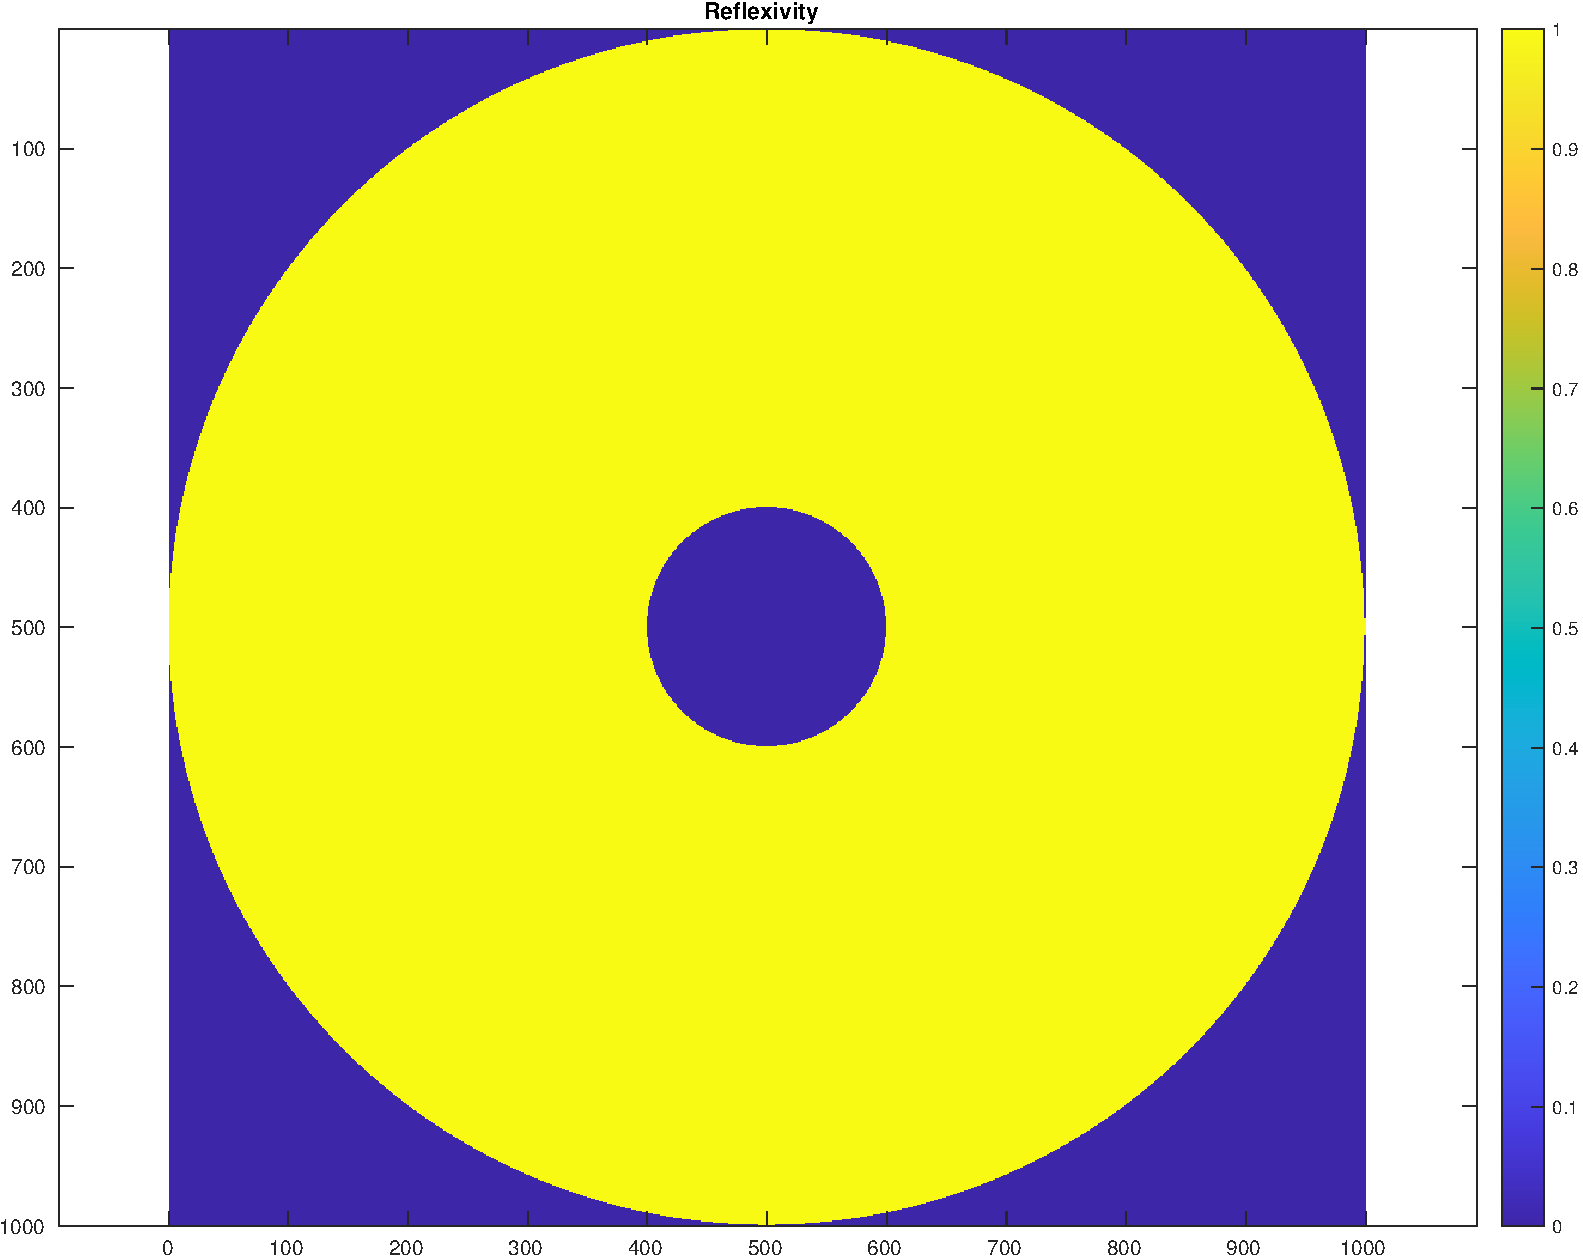
\includegraphics [width=4in]{docuPupilClass_04.pdf}
\begin{par}
Let's add spider : we need to define a spider structure. if it's a simple geometry (line going through the center) it's automatic but the user can define his own mask
\end{par} \vspace{1em}
\begin{verbatim}
SPIDER.n=3; % number of lines
SPIDER.angle=[0 pi/3 2*pi/3]; % angle of each line
SPIDER.width=0.1; % in meter
SPIDER.usrDefined=0;% boolean to decide if spider are build by pupil or defined by user. If so, user must define his own mask
SPIDER.usrMask=[];

P.mkSpiders(SPIDER);
P.disp('r');
\end{verbatim}

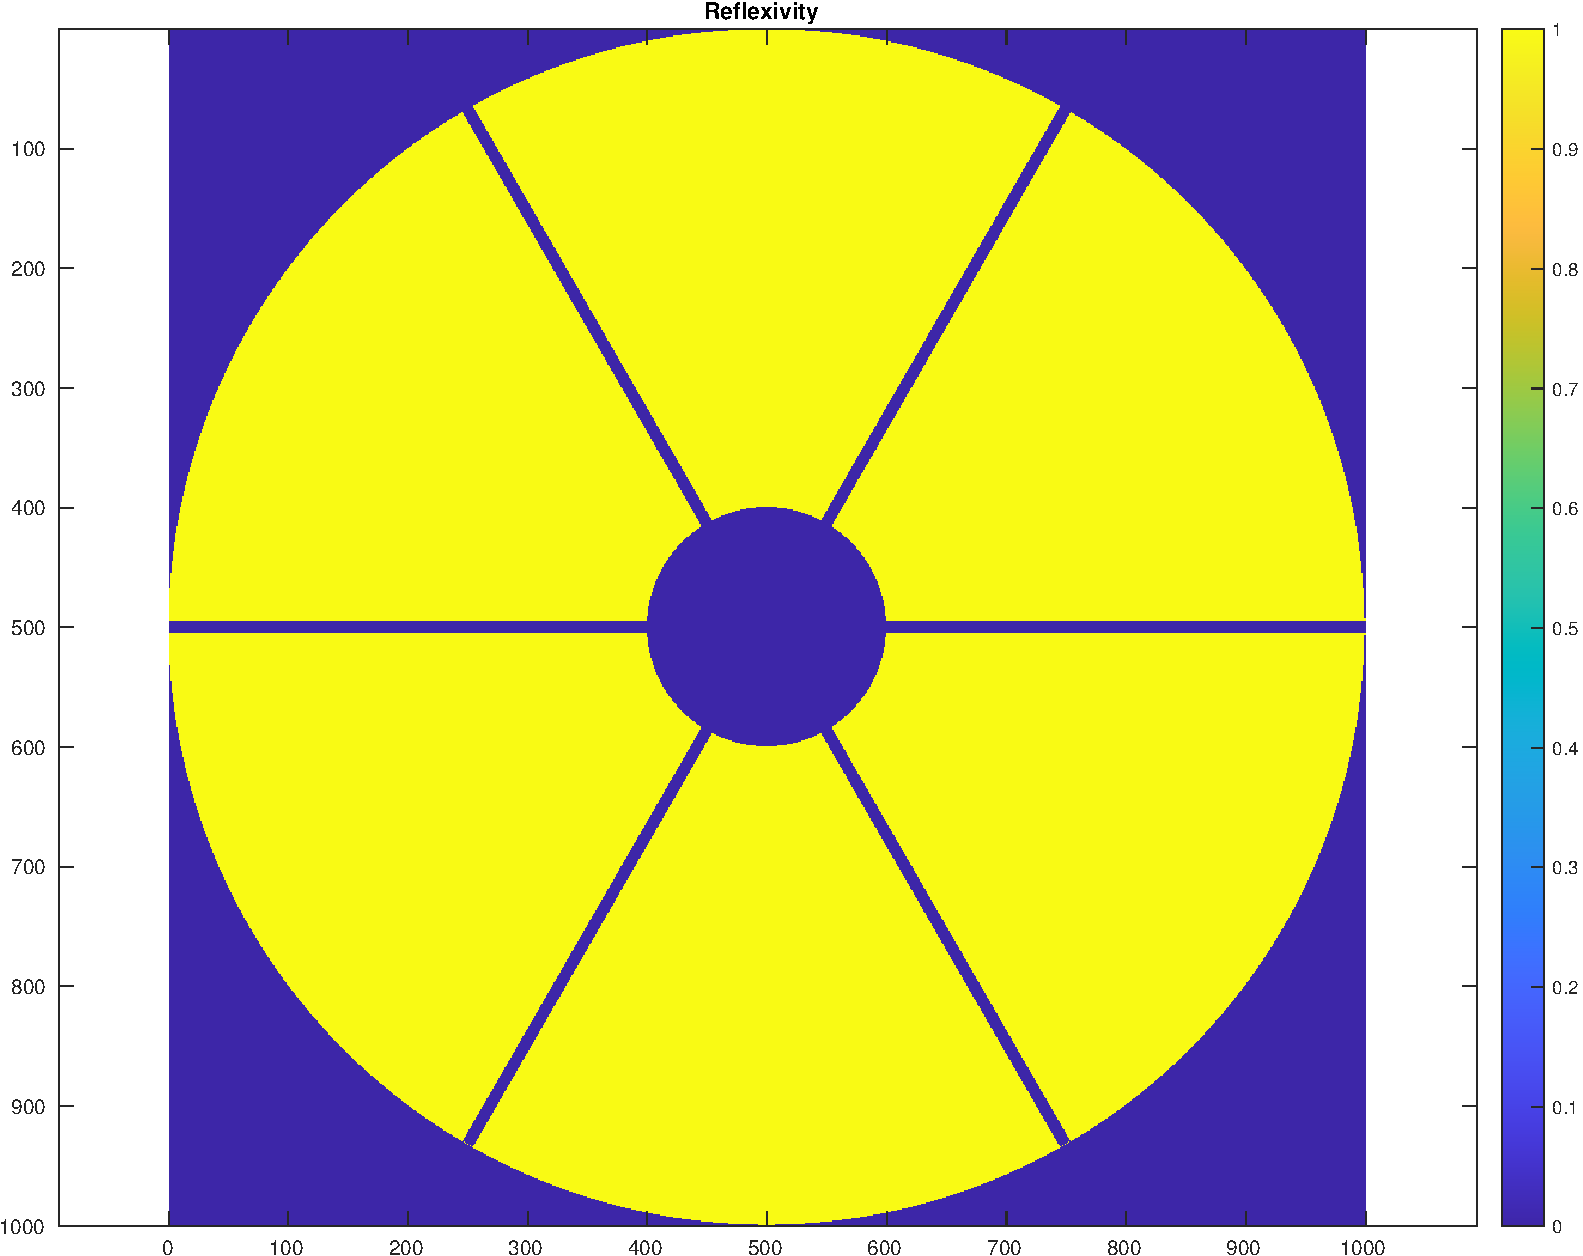
\includegraphics [width=4in]{docuPupilClass_05.pdf}


\subsection*{Segmented Telescopes}

\begin{par}
Let's create a segmented telescope, the Keck, for example. We need a segment of reference, a list of coordinates (in meters or pixels) and a wavelength (important to create the phase). I will now work with pixels.
\end{par} \vspace{1em}
\begin{par}
Note that those coordinates are "optimised" for segments of 200px exactly The fact is that segments are not perfect : for exemple, the up-left side of an hexagon does not perfectly fit the down-right side, so we cannot perfectly mesh the pupil. We need to avoid overlapping segments, but we must also minimize the gaps between each segment. We also need to have a regular mesh to be able to fill the remaining gaps. Thats why it is "easier" to work in pixels. We can adjust  manually the position of each segment, with one pixel precision.
\end{par} \vspace{1em}
\begin{par}
Segments are ordered by their apparition in the coordinates list
\end{par} \vspace{1em}
\begin{verbatim}
SVpx=[   772         535;
         622         448;
         472         535;
         472         709;
         622         796;
         772         709;
         922         448;
         772         361;
         622         274;
         472         361;
         322         448;
         322         622;
         322         796;
         472         883;
         622         970;
         772         883;
         922         796;
         922         622;
        1072         361;
         922         274;
         772         187;
         622         100;
         472         187;
         322         274;
         172         361;
         172         535;
         172         709;
         172         883;
         322         970;
         472        1057;
         622        1144;
         772        1057;
         922         970;
        1072         883;
        1072         709;
        1072         535];
\end{verbatim}
\begin{par}
Of course it is easier to load a .txt ...
\end{par} \vspace{1em}
\begin{verbatim}
S=segment(6,0.9,200);
lambda=2.12e-6;
P=pupil('segRef',S,'segCoord',SVpx,'wavelength',lambda,'unit','px');
\end{verbatim}
\begin{par}
DO NOT forget to specify the unit ! (or expect to have memory issue... Here, the max coordinate is 1134. If the class thinks it's in meter, it will create a HUGE matrix)
\end{par} \vspace{1em}
\begin{verbatim}
P.disp('r');
\end{verbatim}

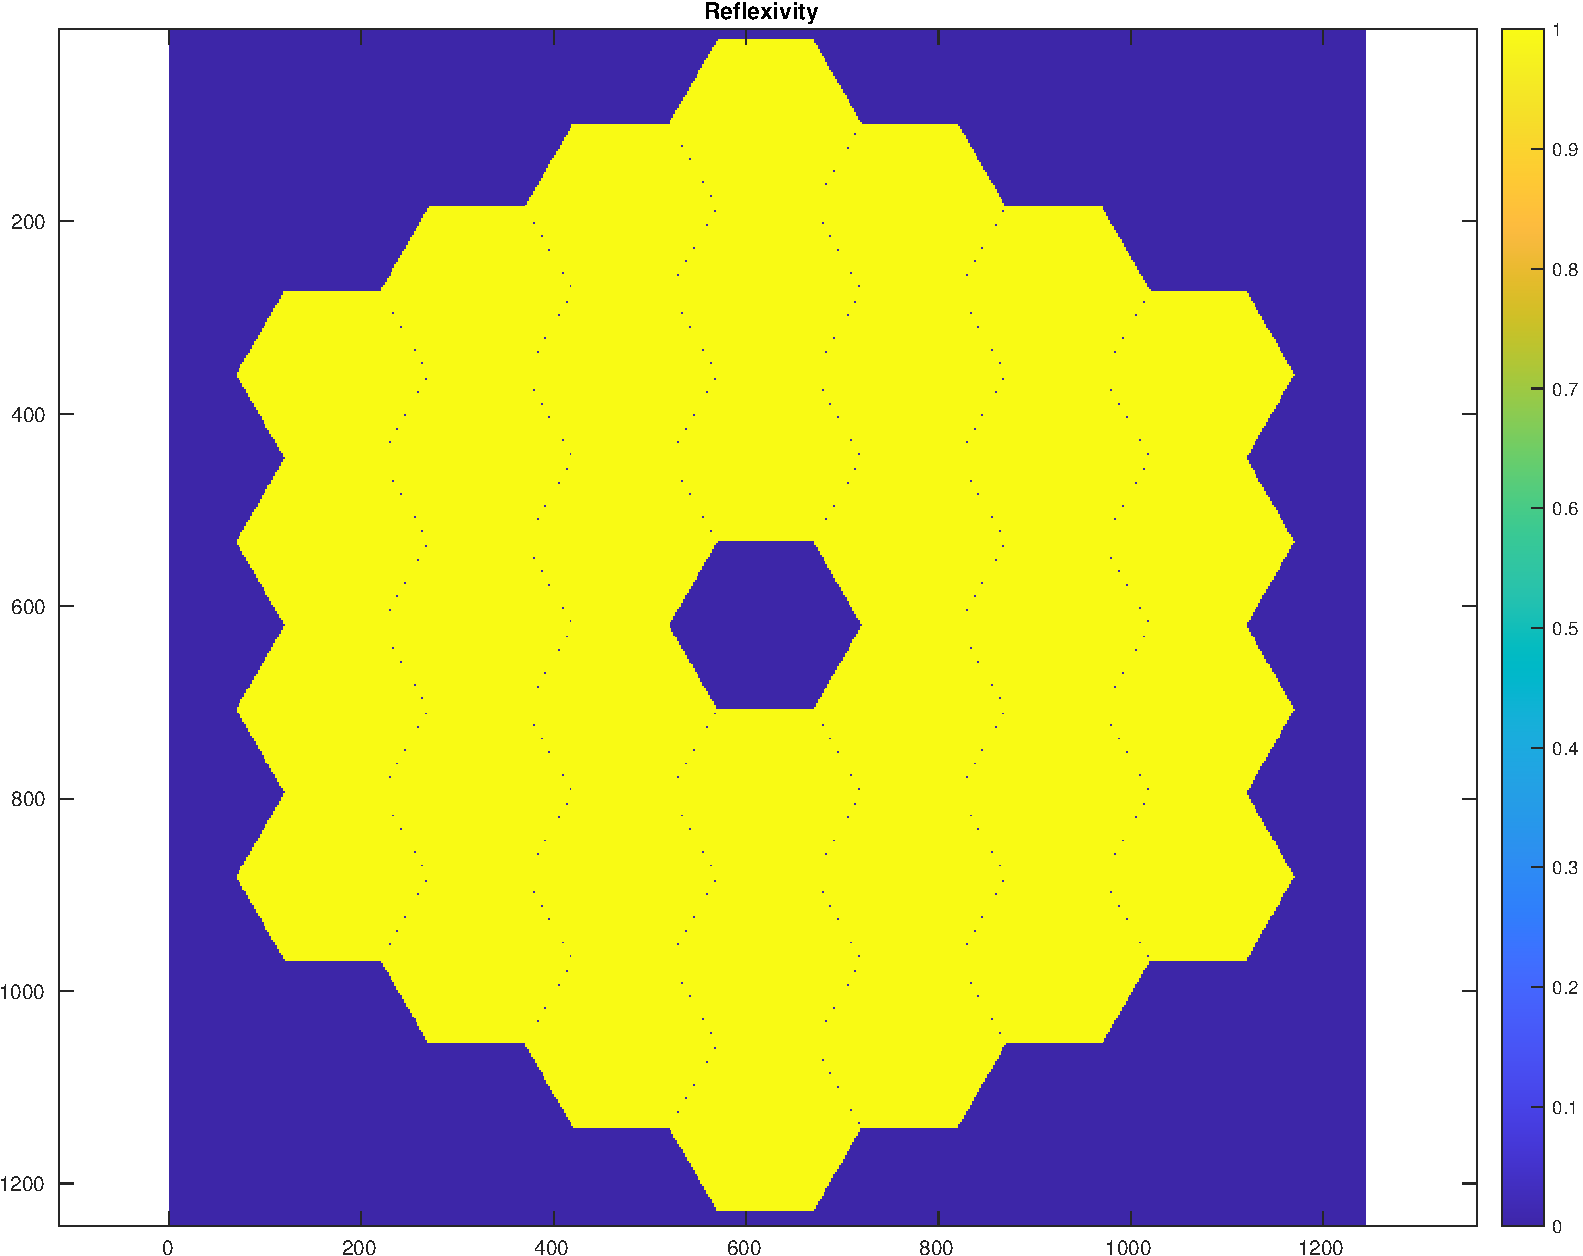
\includegraphics [width=4in]{docuPupilClass_06.pdf}


\section{Pupil including phase and amplitude errors}

\subsection{Introducing Phase and Reflexivity errors}

\begin{par}
Phase : only specify the coefficients and the type of modes (Zernike by default). It's a  [number of segments  x  number of Modes]   matrix.
\end{par} \vspace{1em}
\begin{par}
Reflexivity : an arrow of nSegments giving reflexivity value. It could be a "cube" [segDefinition x segDefinition x number of segment] but it has not been tested yet.
\end{par} \vspace{1em}
\begin{verbatim}
R=0.9+rand(1,length(SVpx))*(1-0.9); % random reflexivity btw .85 and 1

piston=rand(1,length(SVpx))*25e-9; % random piston btw 0 and 25 nm
tip=rand(1,length(SVpx))*10e-9; % random tip btw 0 and 10 nm
tilt=rand(1,length(SVpx))*10e-9; % random tilt btw 0 and 10 nm
focus=rand(1,length(SVpx))*5e-9; % random focus
astig1=rand(1,length(SVpx))*5e-9; % random astig
astig2=rand(1,length(SVpx))*5e-9;

PE=[piston' tip' tilt' focus' astig1' astig2'];

P=pupil('segRef',S,'segCoord',SVpx,'wavelength',lambda,'unit','px',...
    'coeffReflexion',R,'coeffPhaseModes',PE);

P.disp
\end{verbatim}

        \color{lightgray} \begin{verbatim} @(zernike polynomials)> Created!
___ ZERNIKE POLYNOMIALS ___
 . 6 modes: 1,2,3,4,5,6
----------------------------------------------------
 @(zernike polynomials)> Terminated!
\end{verbatim} \color{black}
    
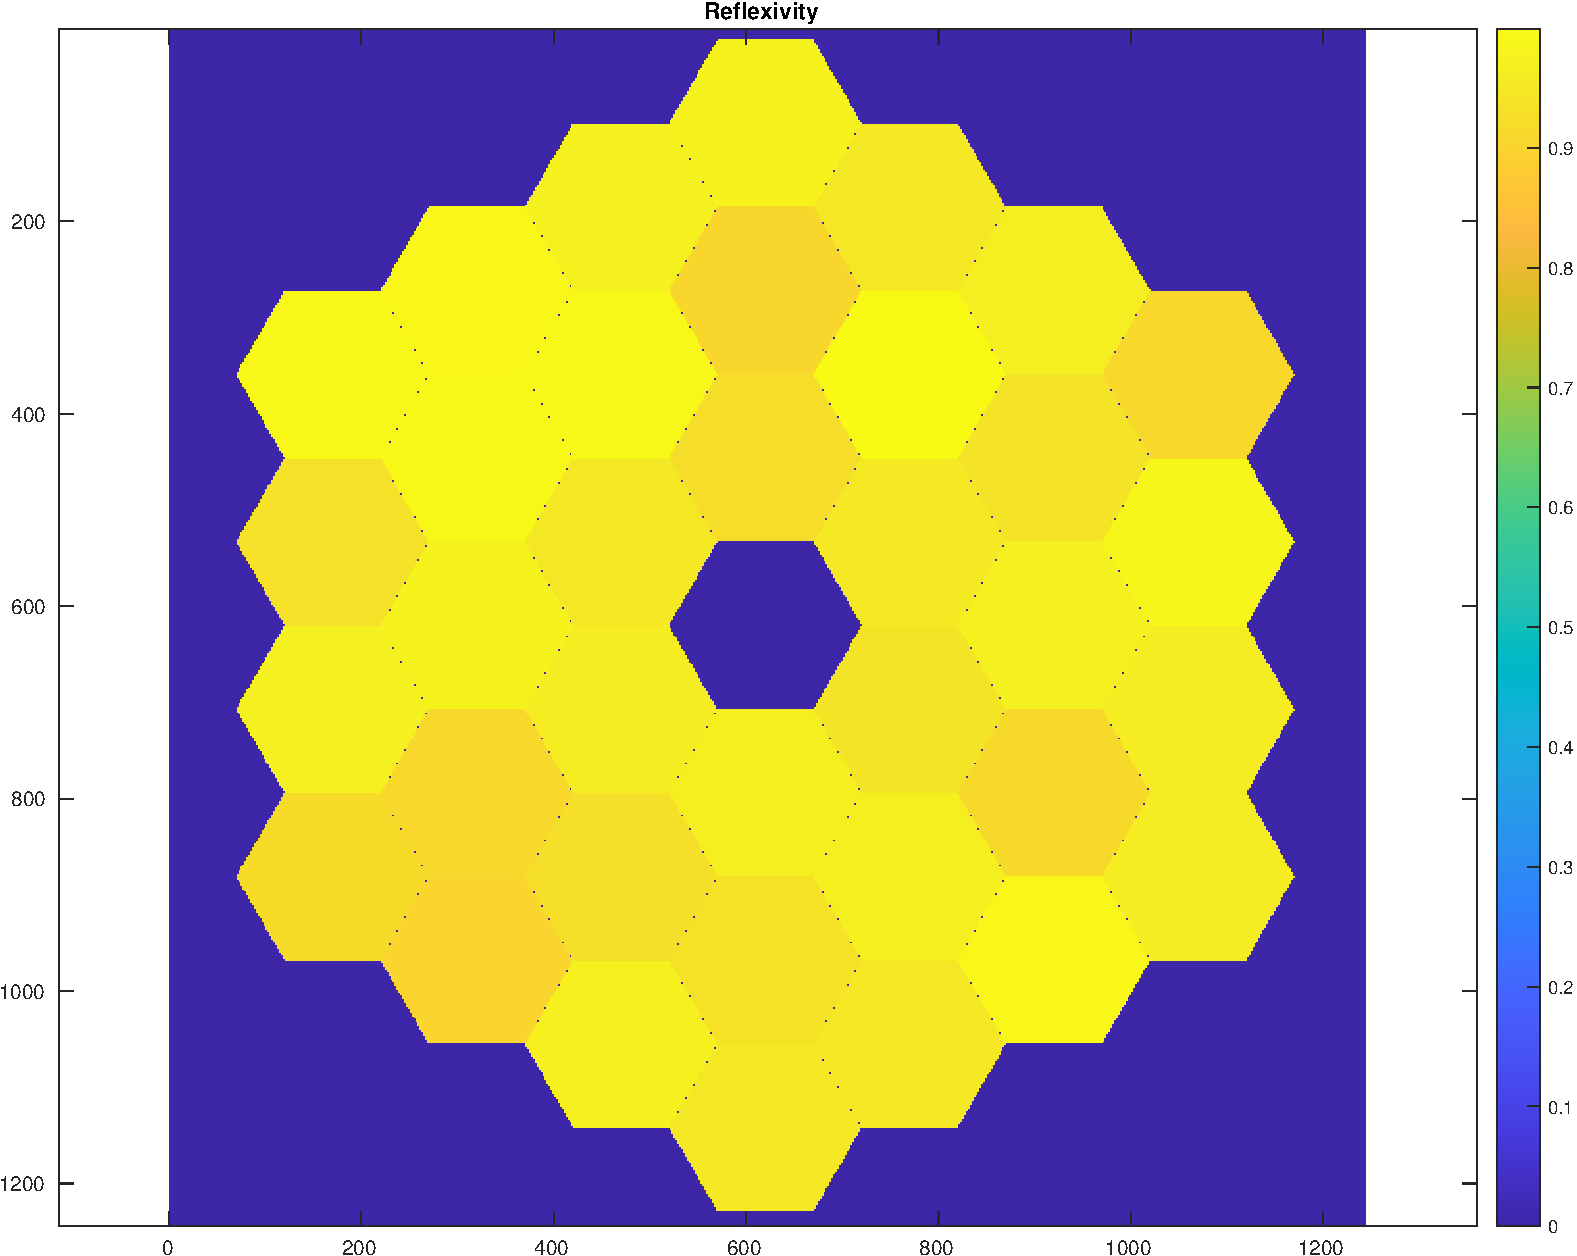
\includegraphics [width=4in]{docuPupilClass_07.pdf}

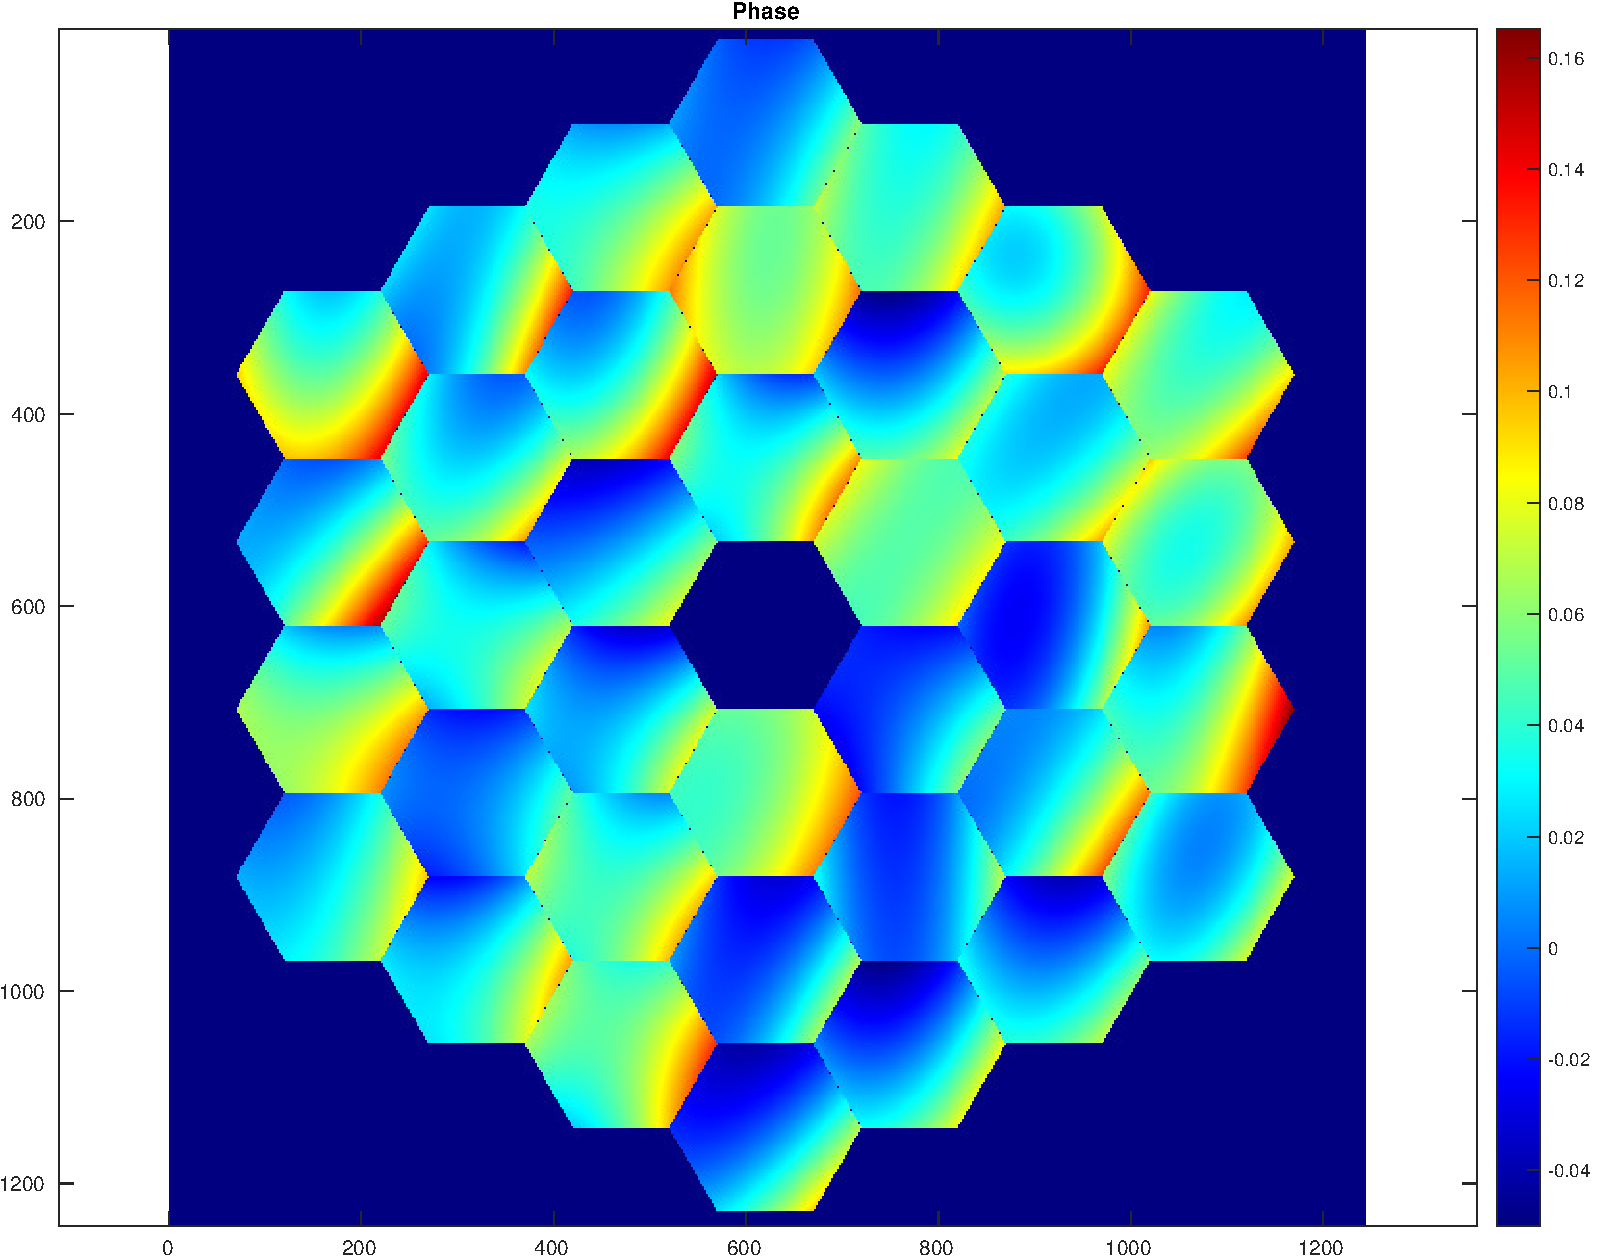
\includegraphics [width=4in]{docuPupilClass_08.pdf}
\begin{par}
Also available by calling P.applyReflexivity and P.applyPhaseError :
\end{par} \vspace{1em}
\begin{par}
segment n°1 and 5 will have a reflexivity of 0.25 and 0.443 respectively
\end{par} \vspace{1em}
\begin{verbatim}
P.applyReflexivity([1 5],[0.25 0.443]);
\end{verbatim}
\begin{par}
segments n° 1 and 12 will get 8 and 13 nm of coma
\end{par} \vspace{1em}
\begin{verbatim}
P.applyPhaseError([1 12], [0 0 0 0 0 0 8; 0 0 0 0 0 0 13]*1e-9);


P.disp;
\end{verbatim}

        \color{lightgray} \begin{verbatim} @(zernike polynomials)> Created!
___ ZERNIKE POLYNOMIALS ___
 . 7 modes: 1,2,3,4,5,6,7
----------------------------------------------------
 @(zernike polynomials)> Terminated!
\end{verbatim} \color{black}
    
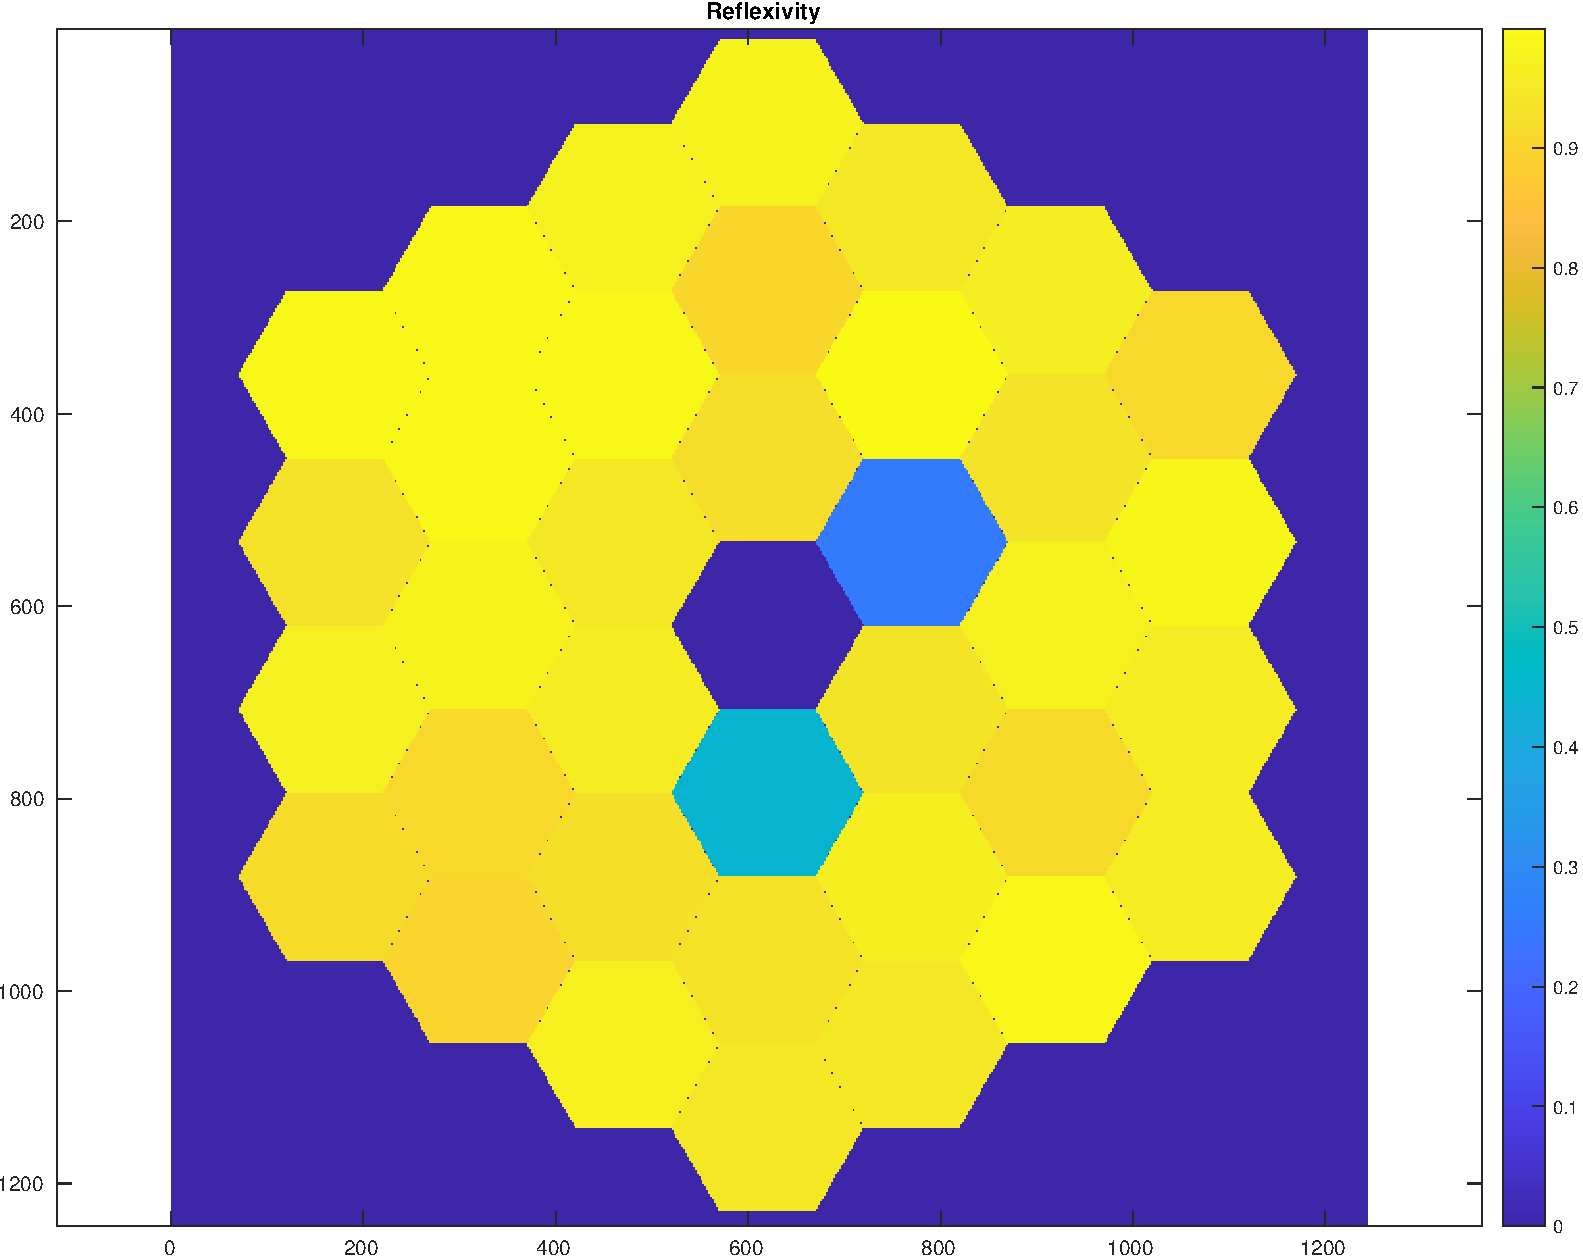
\includegraphics [width=4in]{docuPupilClass_09.pdf}

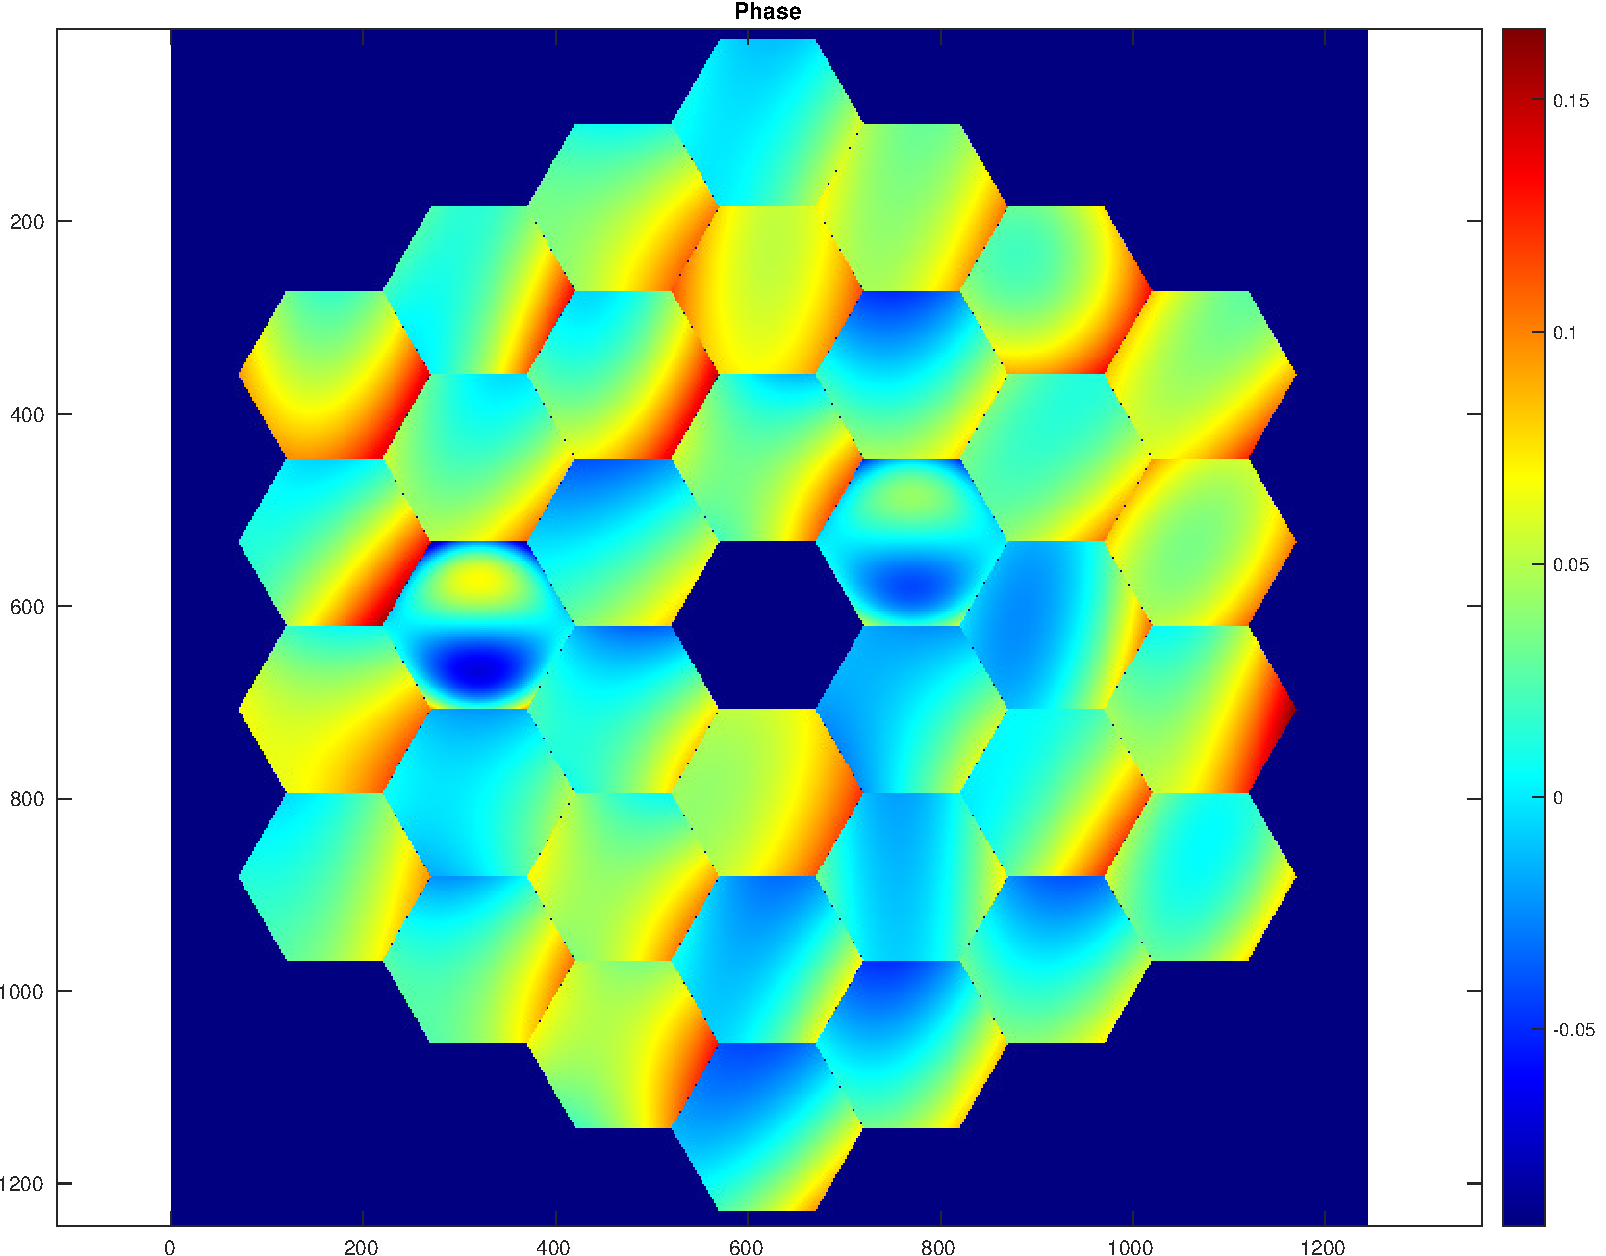
\includegraphics [width=4in]{docuPupilClass_10.pdf}


\subsection*{Geometry Errors}

\begin{par}
Operations available :
\end{par} \vspace{1em}
\begin{itemize}
\setlength{\itemsep}{-1ex}
   \item Shift the segment giving X and Y displacement. Those values will be stored in segment.posXError and segment.posYError /!\ensuremath{\backslash} Warning : x-axis = left to right, y-axis = down to top
\end{itemize}
\begin{itemize}
\setlength{\itemsep}{-1ex}
   \item Rotate the segment giving an angle. The rotation value is stored in  segment.angleError
\end{itemize}
\begin{itemize}
\setlength{\itemsep}{-1ex}
   \item Shrink segment giving a scale factor between 0 and 1. This factor is stored in segment.sizeError
\end{itemize}
\begin{par}
Please be careful : always give the value in the unit used at pupil creation (px or meter)
\end{par} \vspace{1em}
\begin{verbatim}
% move segment n°36 of -300 px on x and -15px on y
% and then rotate it of pi/6 rad
P.shiftSegment(30,-315,-25);
P.rotateSegment(30,pi/6);
P.shrinkSegment(2,0.5); % segment 2 will be shrink at 0.5* original size

P.disp('r');
\end{verbatim}

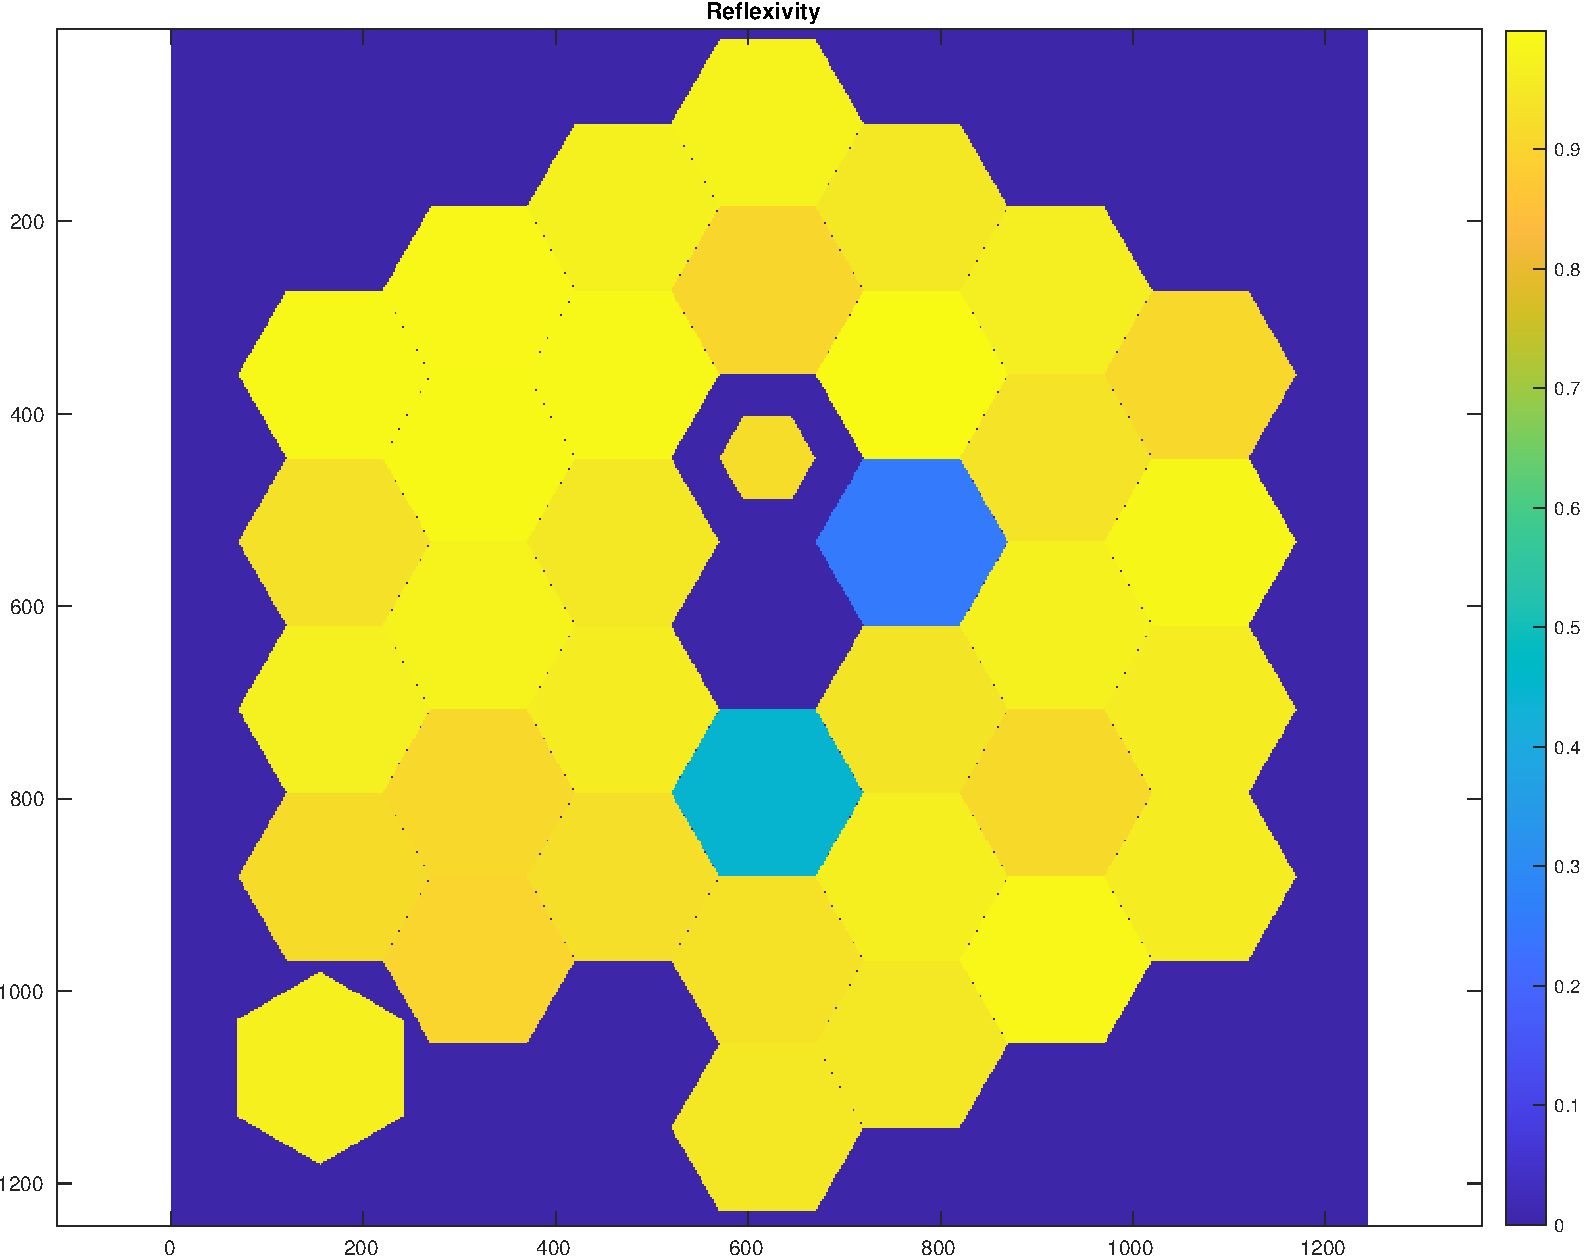
\includegraphics [width=4in]{docuPupilClass_11.pdf}


\subsection*{Modifying the pupil}

\begin{par}
You can zeroPad, remove the borders and resize
\end{par} \vspace{1em}
\begin{itemize}
\setlength{\itemsep}{-1ex}
   \item ZeroPad : add zeros around the pupil for sampling purposes (frequency domain), giving  a coefficient
\end{itemize}
\begin{itemize}
\setlength{\itemsep}{-1ex}
   \item removeZeroBorder : remove all the border full of zeros, but keep the matrix square
\end{itemize}
\begin{itemize}
\setlength{\itemsep}{-1ex}
   \item resize : resize the pupil giving a new number of pixels. It is using interp2 Matlab function, so you can specify the method (linear, nearest,spline,cubic). Nearest, by default, seems to be the best method (no strange pixel in reflexivity nor phase)
\end{itemize}
\begin{par}
Those methods will produce a temporary matrix and will change the pupil matrix. If you want only the tmp matrix but do not want the original pupil to be modified, you can specify 0 or 1 after the main arguments
\end{par} \vspace{1em}
\begin{par}
Please note that rmZeroBorder and Resize prevent you from modifying the pupil : all the methods (geometry, reflexivity and phase) are based on the segments geometry. As we resize the whole pupil matrix and not each segment one by one, trying the methods above will produce weird results
\end{par} \vspace{1em}
\begin{par}
Original Matrix
\end{par} \vspace{1em}
\begin{verbatim}
P.disp('r');
\end{verbatim}

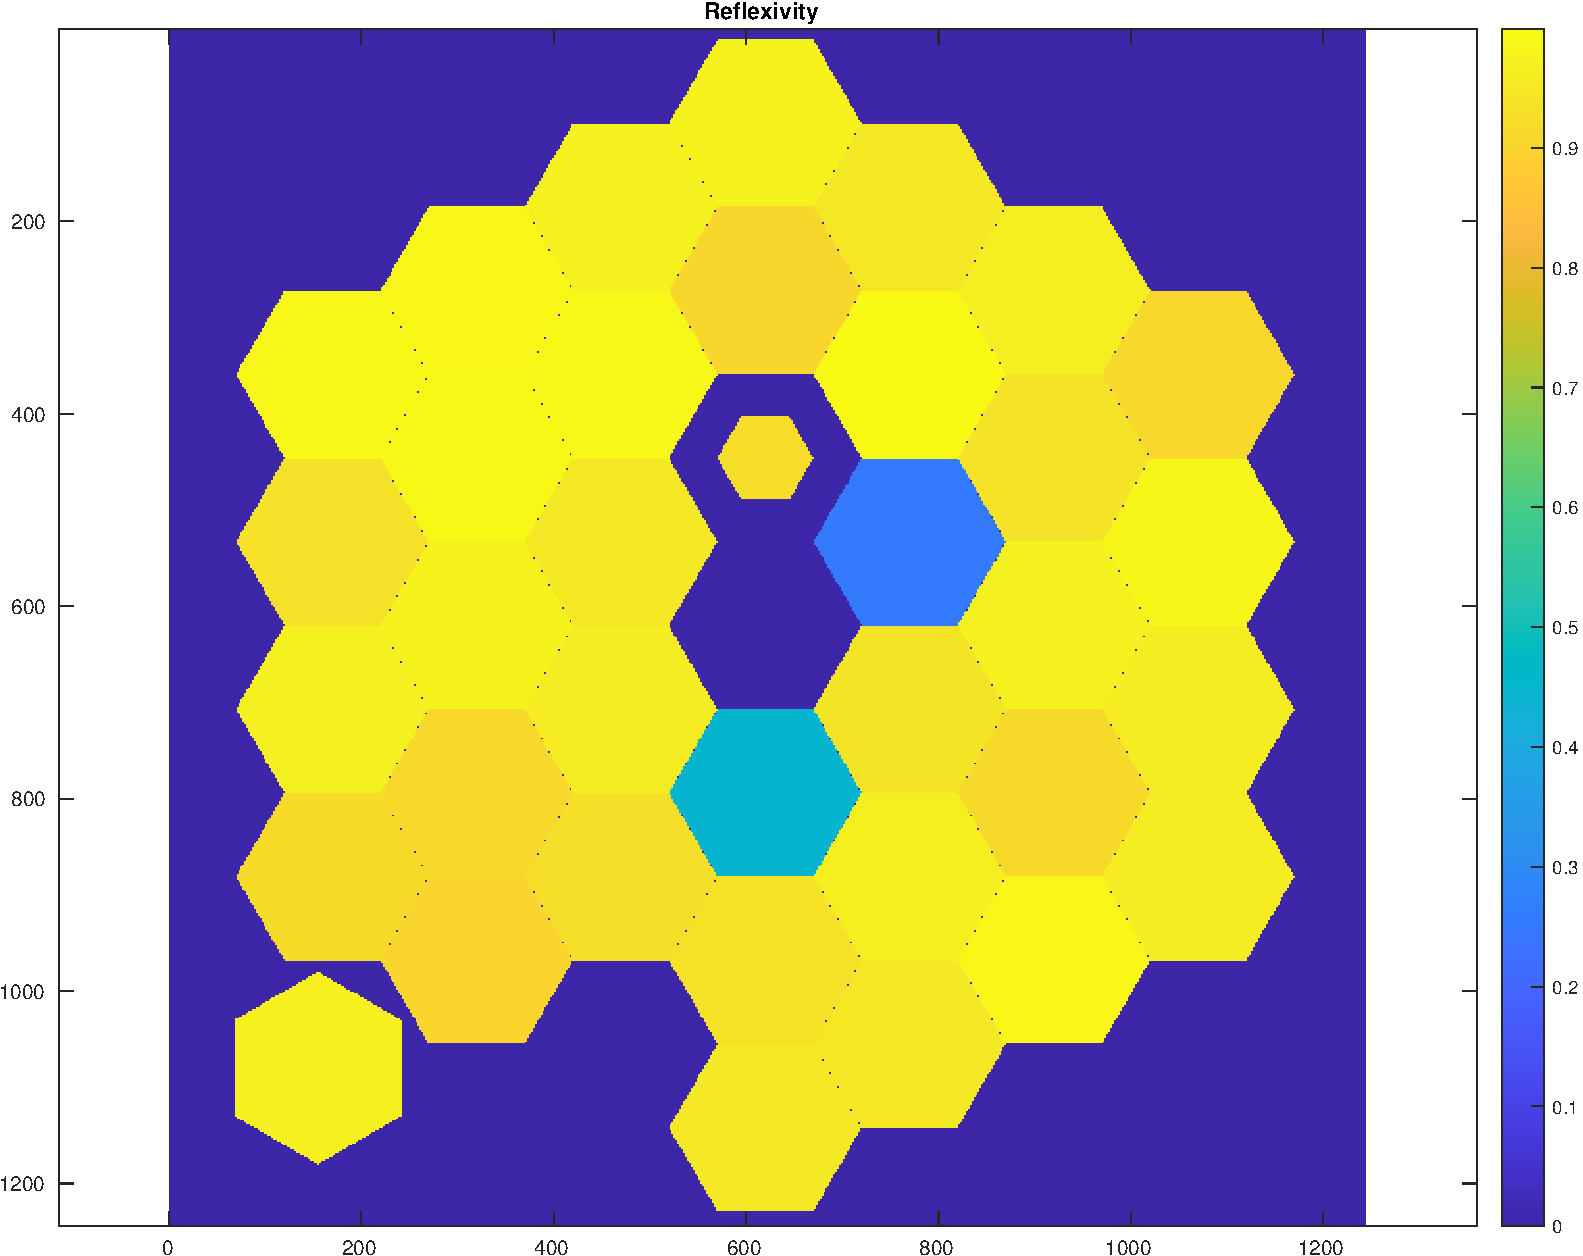
\includegraphics [width=4in]{docuPupilClass_12.pdf}
\begin{par}
Removing empty border
\end{par} \vspace{1em}
\begin{verbatim}
tmpMat=P.rmZeroBorder(0); % flagReplace at 0 -> you'll get the tmp Matrix in  tmpMatrix but the original pupil will not be modified


P.rmZeroBorder(1); % flagReplace at 1 -> pupil will be modified inside the object
P.disp('r');
\end{verbatim}

        \color{lightgray} \begin{verbatim}removing border full of zeros
removing border full of zeros
\end{verbatim} \color{black}
    
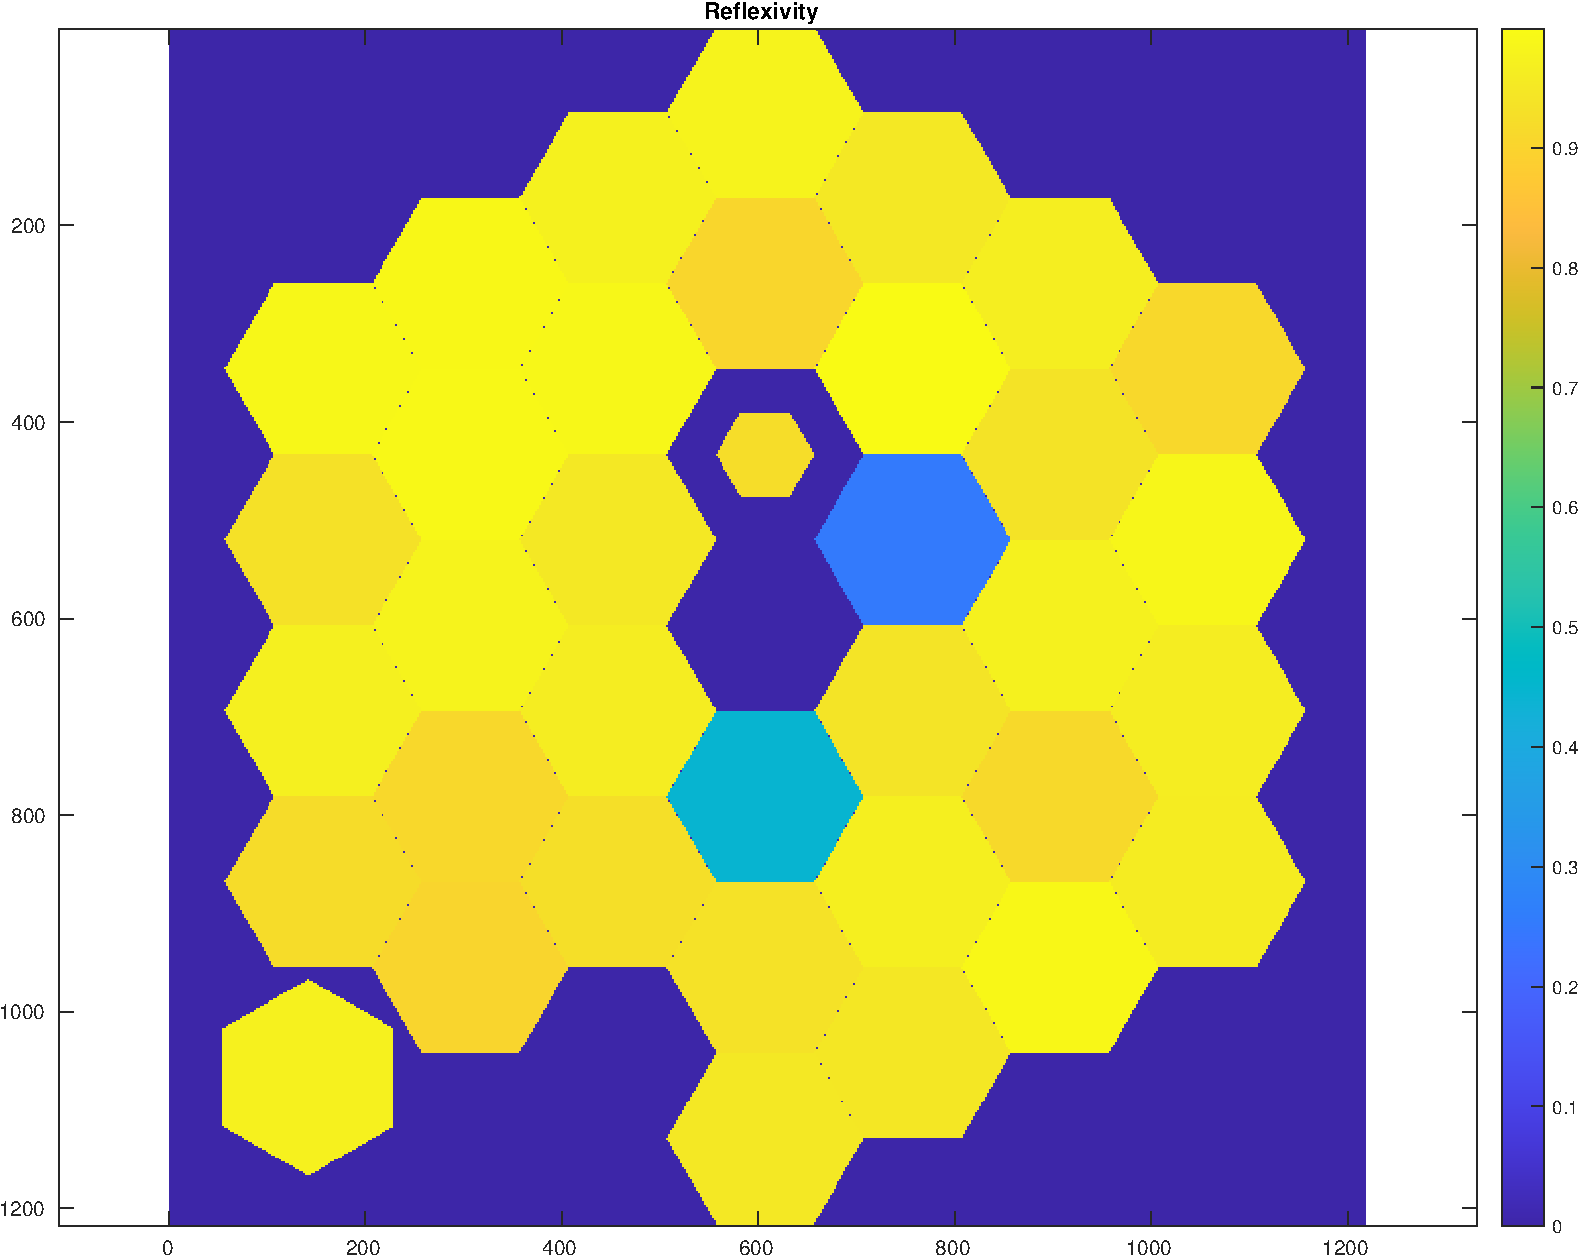
\includegraphics [width=4in]{docuPupilClass_13.pdf}
\begin{par}
ZeroPad
\end{par} \vspace{1em}
\begin{verbatim}
P.zeroPad(2,1); % pupil will be 2x larger -> Nyquist sampling in frequency domainP.disp('r');
P.disp('r');
\end{verbatim}

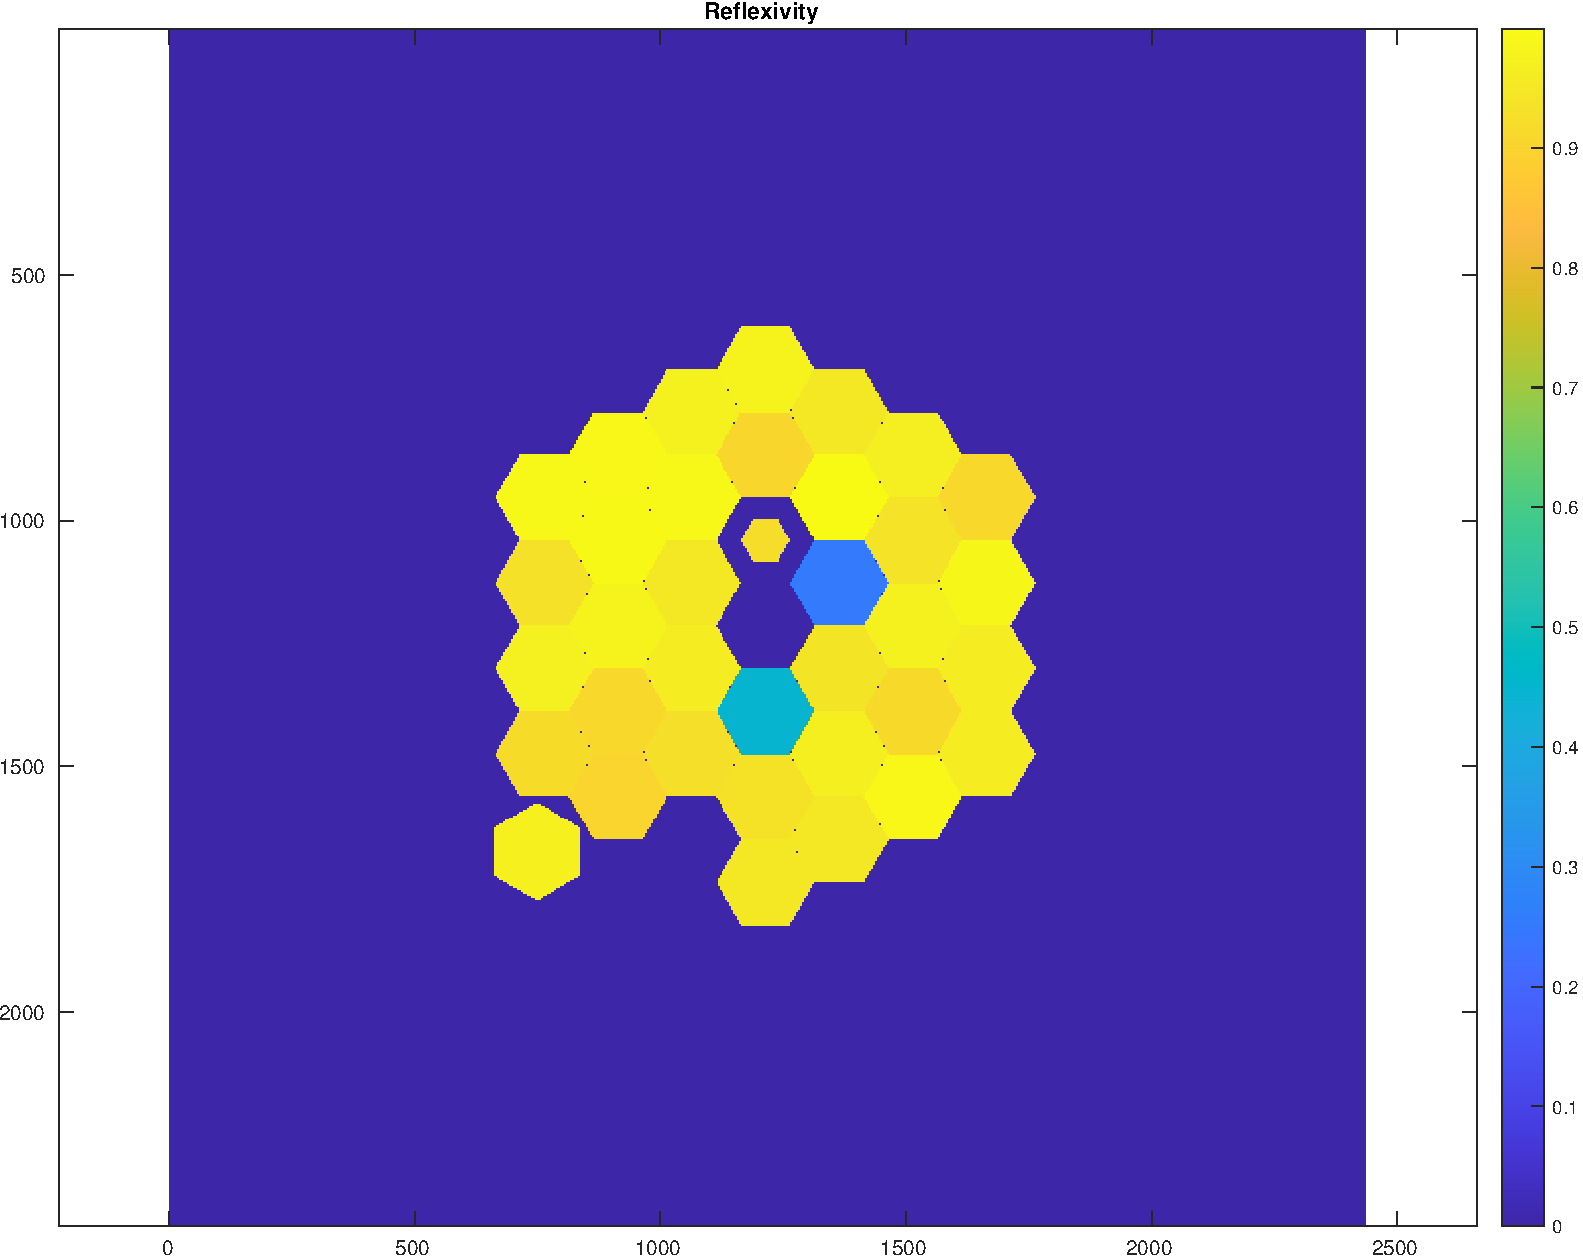
\includegraphics [width=4in]{docuPupilClass_14.pdf}
\begin{par}
Resize
\end{par} \vspace{1em}
\begin{verbatim}
P.resize(600,1,'nearest'); % pupil will be resized at 300px, replaced in the object, using Nearest Neighbor interpolation
P.disp('r');
\end{verbatim}

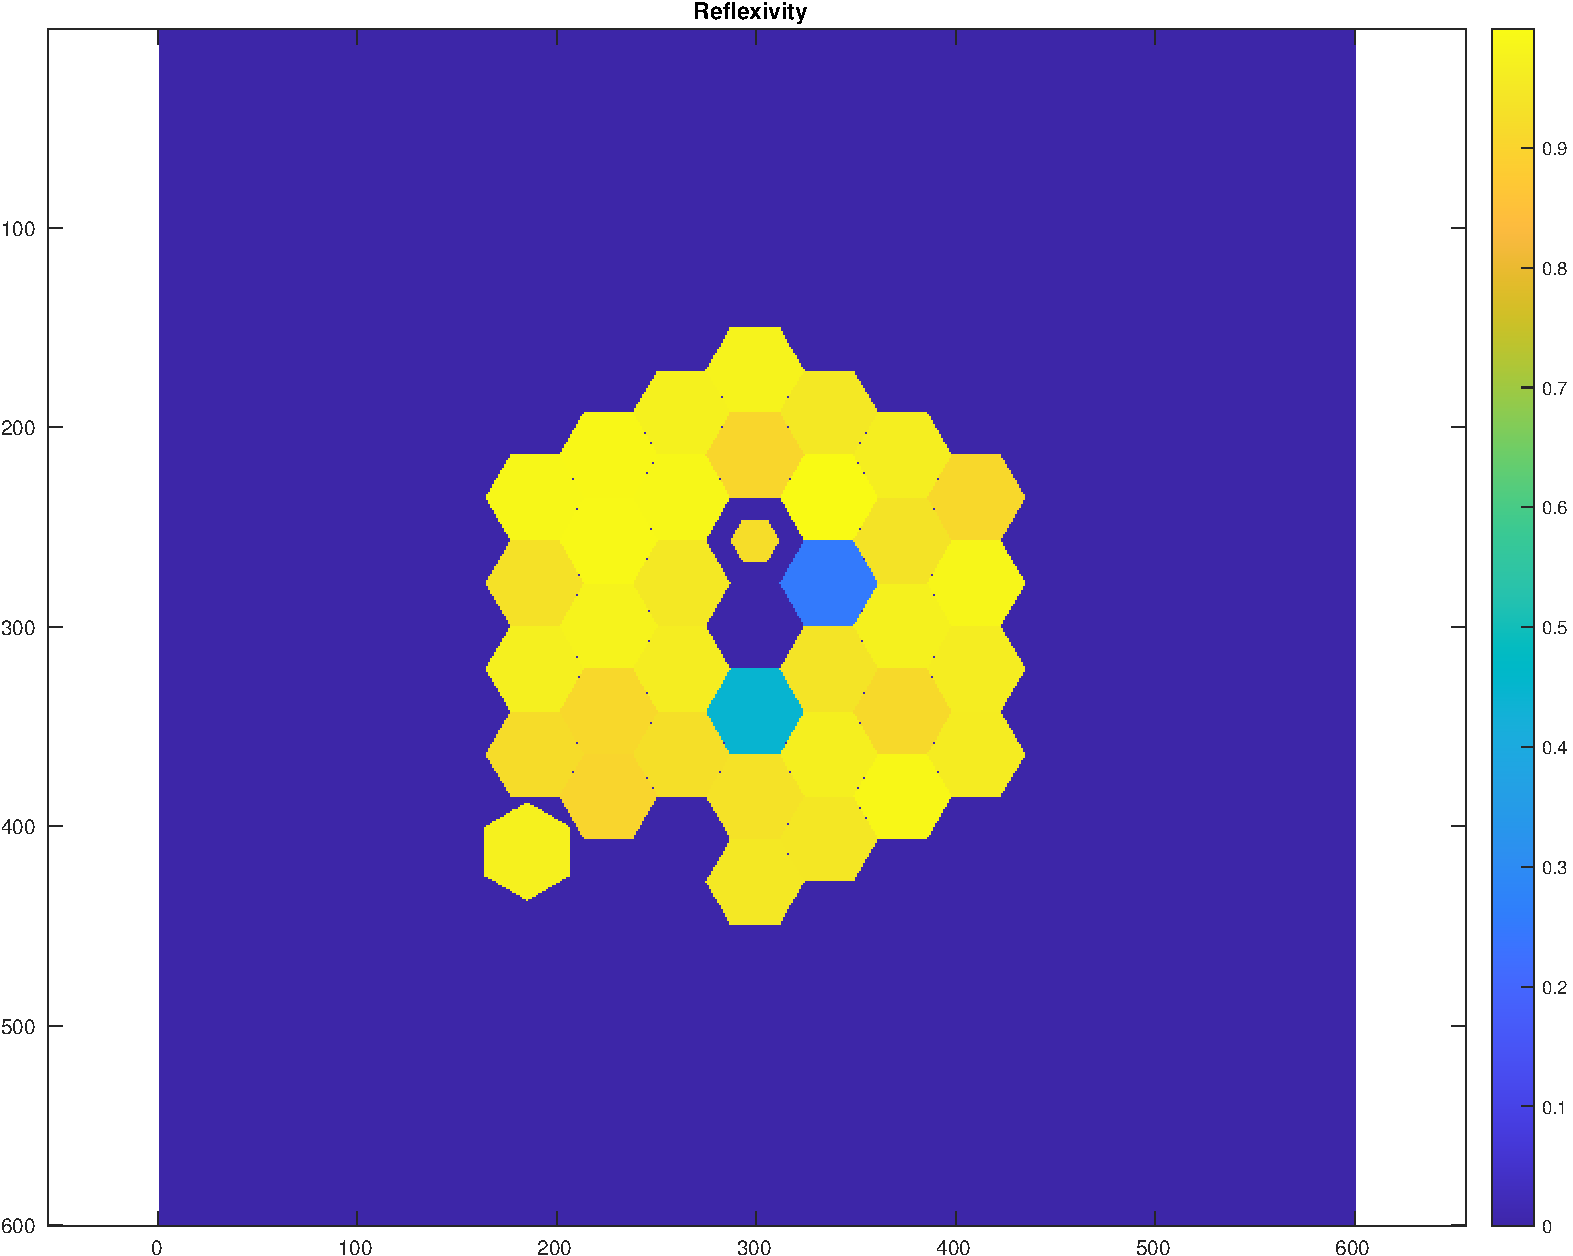
\includegraphics [width=4in]{docuPupilClass_15.pdf}


\subsection{Filling the gaps}

\begin{par}
As said above, the segment class does not produce good shape for meshing. Moreover, if coordinates are given in meters, the conversion meters-\ensuremath{>} pixels could produce rounding errors. Consequences : pixels may overlap, or create gaps between segments.
\end{par} \vspace{1em}
\begin{par}
Solution : create "optimized" coordinates in pixel for a given segment size. They must avoid overlapping pixels, but be as "tight" as possible (= a few gaps as possible). The segments must be regulary placed. Example :
\end{par} \vspace{1em}

\begin{verbatim}  1   2  3
1     O
2  O     O
3     O
4  O     O
5     O\end{verbatim}
    \begin{par}
in the scheme above :
\end{par} \vspace{1em}

\begin{verbatim}segment(2,3) = segment(2,1)+[0 segDiameter]
segment(4,3) = segment(4,1)+[0 segDiameter]
segment(4,1) = segment(2,1)+[segHeight 0]
segment(4,3) = segment(2,3)+[segHeight 0]
segment(1,2) = segment(2,1)+[segHeight/2  cos(30)*segDiameter]
segment(3,2) = segment(4,1)+[segHeight/2  cos(30)*segDiameter]
segment(5,2) = segment(4,1)+[segHeight/2  cos(30)*segDiameter]\end{verbatim}
    \begin{par}
Once it's done, just add the parameter "flagNoGap" at 1.
\end{par} \vspace{1em}
\begin{verbatim}
S=segment(6,0.9,200);
lambda=2.12e-6;
P1=pupil('segRef',S,'segCoord',SVpx,'wavelength',lambda,...
    'flagNoGap',0,'unit','px','coeffReflexion',R,'coeffPhaseModes',PE);

P2=pupil('segRef',S,'segCoord',SVpx,'wavelength',lambda,...
    'flagNoGap',1,'unit','px','coeffReflexion',R,'coeffPhaseModes',PE);

P1.disp('r');
P2.disp('r');
\end{verbatim}

        \color{lightgray} \begin{verbatim} @(zernike polynomials)> Created!
___ ZERNIKE POLYNOMIALS ___
 . 6 modes: 1,2,3,4,5,6
----------------------------------------------------
 @(zernike polynomials)> Terminated!
 @(zernike polynomials)> Created!
___ ZERNIKE POLYNOMIALS ___
 . 6 modes: 1,2,3,4,5,6
----------------------------------------------------
 @(zernike polynomials)> Terminated!
\end{verbatim} \color{black}
    
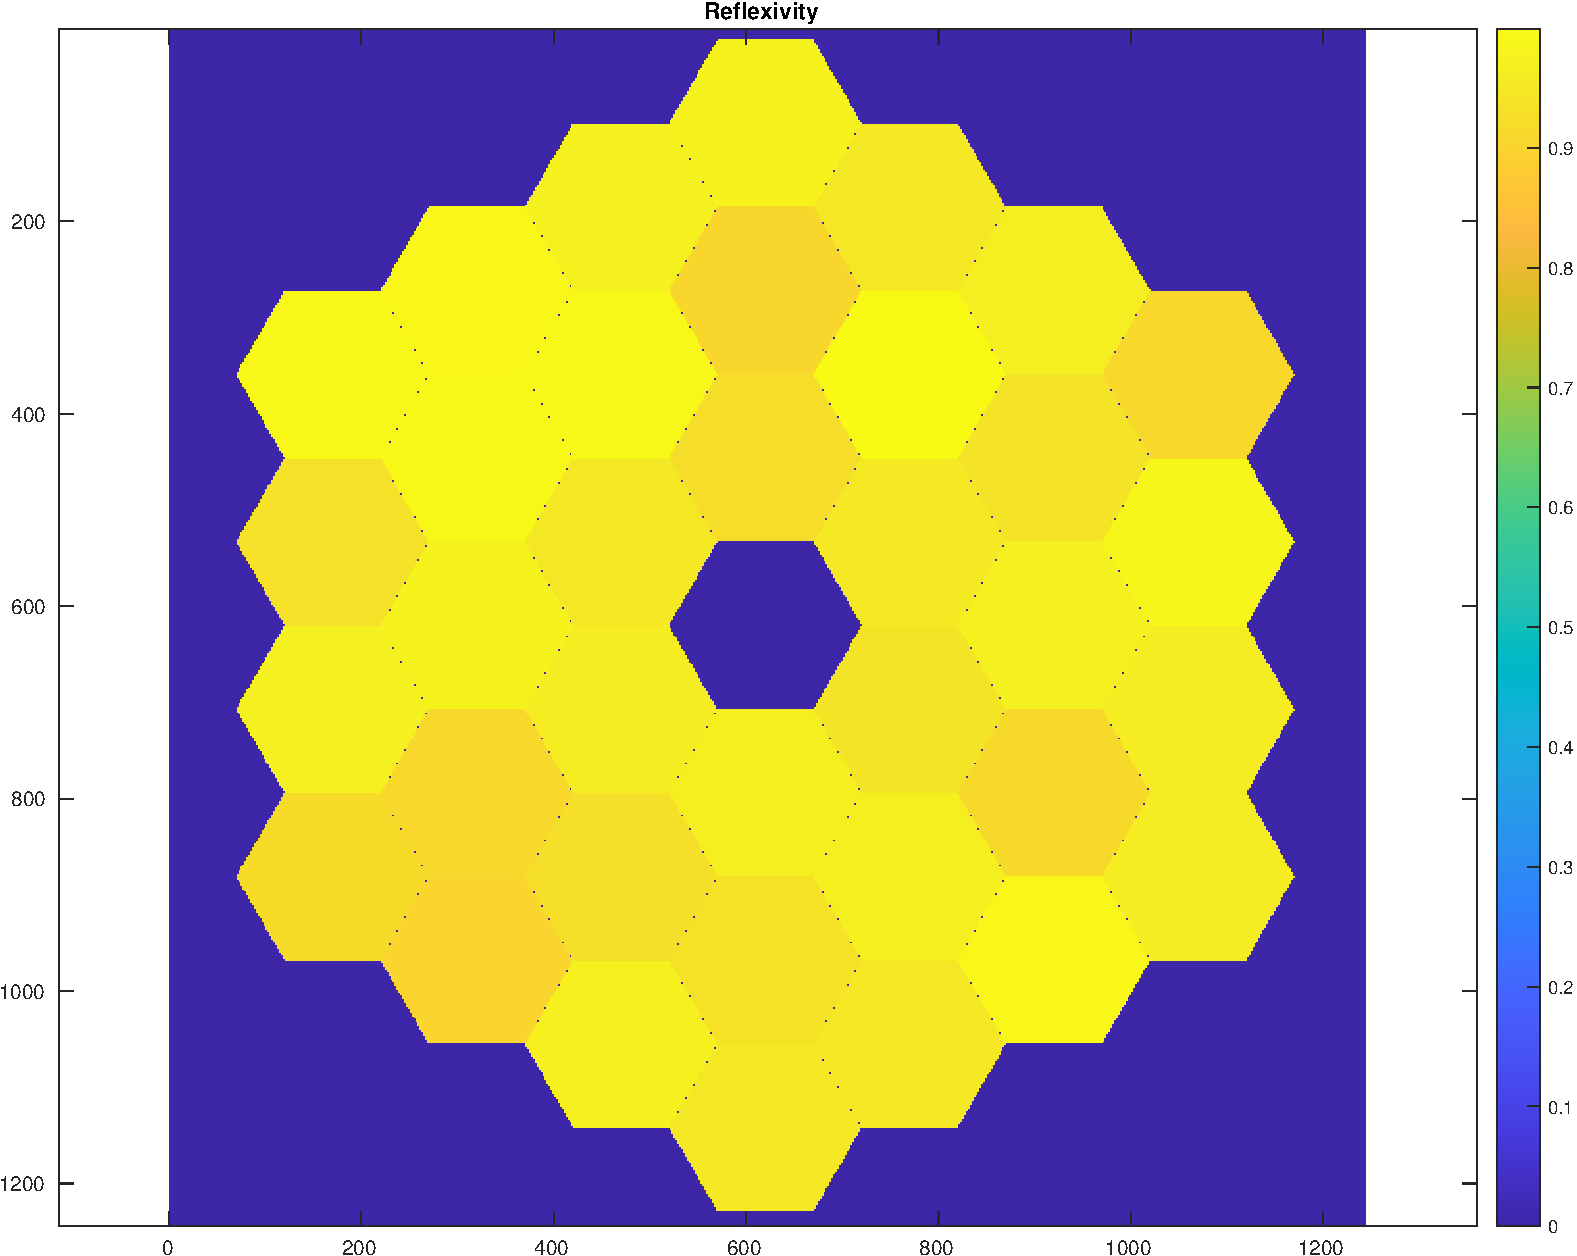
\includegraphics [width=4in]{docuPupilClass_16.pdf}

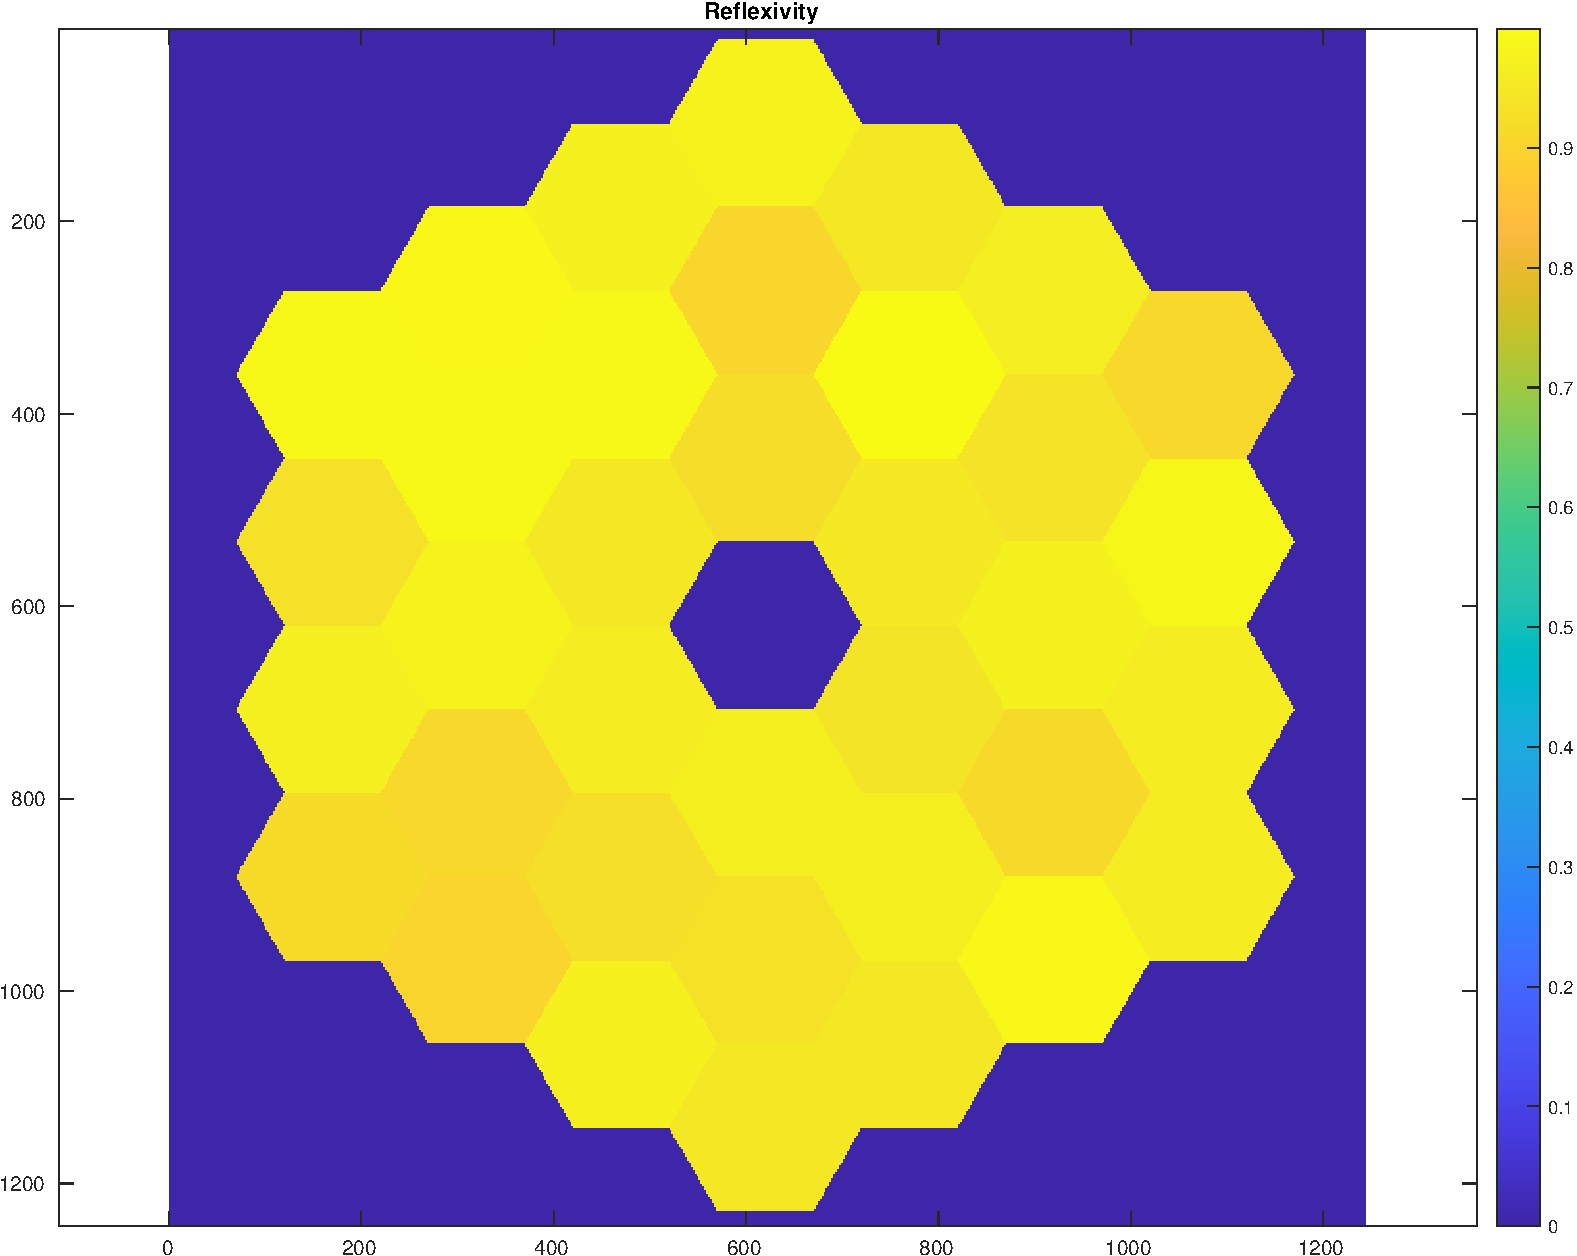
\includegraphics [width=4in]{docuPupilClass_17.pdf}

\section{Application to KECK telescope}

\section{Conclusions}


\bibliographystyle{plain} 
\bibliography{/home/omartin/Documents/Bibliography/biblioLolo}

\end{document}
